\documentclass[12pt,a4paper]{report}

\usepackage[utf8]{inputenc}
\usepackage[romanian,english]{babel}
\renewcommand\familydefault{\sfdefault}

\usepackage[table,xcdraw]{xcolor}
\usepackage[margin=2.54cm]{geometry}
\usepackage{graphicx}

\usepackage{textcase}
\usepackage[titletoc, title]{appendix}
\usepackage{titlesec}
\titleformat{\chapter}{\large\bfseries\MakeUppercase}{\thechapter}{2ex}{}[\vspace*{-1.5cm}]
\titleformat*{\section}{\large\bfseries}
\titleformat*{\subsection}{\large\bfseries}
\titleformat*{\subsubsection}{\large\bfseries}

\usepackage{float}
\usepackage{microtype}
\usepackage{nicefrac}
\usepackage{amsfonts}
\usepackage{url}
\usepackage{multirow}
\usepackage{amssymb,amsmath,amsfonts,amsthm,bm}
\usepackage{tabularx}
\usepackage{listings}

\definecolor{codegray}{rgb}{0.5,0.5,0.5}
\definecolor{backcolour}{rgb}{0.95,0.95,0.92}

\lstdefinestyle{mystyle}{
    backgroundcolor=\color{backcolour},
    numberstyle=\tiny\color{codegray},
    basicstyle=\ttfamily\footnotesize,
    breakatwhitespace=false,
    breaklines=true,
    captionpos=b,
    keepspaces=true,
    numbers=left,
    numbersep=5pt,
    showspaces=false,
    showstringspaces=false,
    showtabs=false,
    tabsize=2
}
\lstset{style=mystyle}

\usepackage{chngcntr}
\counterwithout{figure}{chapter}
\counterwithout{table}{chapter}
\counterwithout{equation}{chapter}

\usepackage{booktabs}
\usepackage[bookmarks,unicode,hidelinks]{hyperref}

\usepackage{array}
\usepackage{paralist}
\usepackage{verbatim}
\usepackage{subfig}
\usepackage{enumitem}
\setlist{noitemsep}

%%% HEADERS & FOOTERS
\usepackage{fancyhdr}
\pagestyle{empty}
\renewcommand{\headrulewidth}{0pt}
\renewcommand{\footrulewidth}{0pt}
\lhead{}\chead{}\rhead{}
\lfoot{}\cfoot{\thepage}\rfoot{}

\newcommand{\HeaderLineSpace}{-0.25cm}
\newcommand{\UniTextRO}{UNIVERSITATEA POLITEHNICA DIN BUCUREȘTI \\[\HeaderLineSpace]
FACULTATEA DE AUTOMATICĂ ȘI CALCULATOARE \\[\HeaderLineSpace]
DEPARTAMENTUL DE CALCULATOARE\\}
\newcommand{\DiplomaRO}{PROIECT DE CERCETARE}
\newcommand{\AdvisorRO}{Coordonator științific:}
\newcommand{\BucRO}{BUCUREȘTI}

\newcommand{\UniTextEN}{UNIVERSITY POLITEHNICA OF BUCHAREST \\[\HeaderLineSpace]
FACULTY OF AUTOMATIC CONTROL AND COMPUTERS \\[\HeaderLineSpace]
COMPUTER SCIENCE AND ENGINEERING DEPARTMENT\\}
\newcommand{\DiplomaEN}{Scientific Report \#3}
\newcommand{\AdvisorEN}{Scientific advisors:}
\newcommand{\BucEN}{BUCHAREST}

\newcommand{\frontPage}[6]{
\begin{titlepage}
\begin{center}
{\Large #1}
\vspace{50pt}
\begin{tabular}{p{6cm}p{4cm}}

\includegraphics[scale=0.8]{figures/upb-logo.jpg} &
	
\includegraphics[scale=0.5,trim={14cm 11cm 2cm 5cm},clip=true]{figures/cs-logo.pdf}
\end{tabular}

\vspace{105pt}
{\Huge #2}\\
\vspace{40pt}
{\Large #3}\\ \vspace{0pt}
{\Large #4}\\
\vspace{40pt}
{\LARGE \Name}\\
\end{center}
\vspace{60pt}
\begin{tabular*}{\textwidth}{@{\extracolsep{\fill}}p{6cm}r}
&{\large\textbf{#5}}\vspace{10pt}\\
&{\large \AdvisorA}\\
&{\large \AdvisorB}
\end{tabular*}
\vspace{20pt}
\begin{center}
{\large\textbf{#6}}\\
\vspace{0pt}
{\normalsize \Year}
\end{center}
\end{titlepage}
}

\newcommand{\frontPageRO}{\frontPage{\UniTextRO}{\DiplomaRO}{\ProjectTitleRO}{\ProjectSubtitleRO}{\AdvisorRO}{\BucRO}}
\newcommand{\frontPageEN}{\frontPage{\UniTextEN}{\DiplomaEN}{\ProjectTitleEN}{\ProjectSubtitleEN}{\AdvisorEN}{\BucEN}}

\linespread{1.15}
\setlength\parindent{0pt}
\setlength\parskip{.28cm}

\newcommand{\AbstractPage}{
\begin{titlepage}
\textbf{\large ABSTRACT}\par
\AbstractEN \vfill
\end{titlepage}
}

\tolerance=1
\emergencystretch=\maxdimen
\hyphenpenalty=10000
\hbadness=10000
\sloppy

%%%%%%%%%%%%%%%%%%%%%%%%%%%%%%%%%%%%%%%%%%%%%%%%%%

\newcommand{\ProjectTitleRO}{Un studiu empiric al strategiilor de antrenare pentru generalizarea în afara domeniului în Aspect-Based Sentiment Analysis}
\newcommand{\ProjectSubtitleRO}{Programul de master IISC}
\newcommand{\ProjectTitleEN}{A Systematic Empirical Study of Training Strategies for Out-of-Domain Generalisation in Generative Aspect-Based Sentiment Analysis}
\newcommand{\ProjectSubtitleEN}{Master Program IISC}
\newcommand{\Name}{[TO DO]}
\newcommand{\AdvisorA}{[TO DO]}
\newcommand{\AdvisorB}{}
\newcommand{\Year}{2025}

\title{Raport de cercetare}
\author{\Name}
\date{\Year}

\newcommand{\AbstractEN}{This report presents an empirical study of training strategies for out-of-domain generalisation in generative Aspect-Based Sentiment Analysis. We formulate Aspect Sentiment Triplet Extraction as a sequence-to-sequence problem using FLAN-T5-base and systematically evaluate the effect of output format, syntactic input enrichment, multi-ordering training, mixed-objective training, curriculum learning, aspect masking, cross-domain data mixing, and decoding strategies on cross-domain performance. Experiments are conducted on the SemEval ASTE benchmark (restaurant to laptop transfer) and the DMASTE multi-domain benchmark, with multi-seed statistical validation. Our main finding is that natural-language output templates provide the largest improvement for OOD generalisation (+8.6 F1 over structured output, 5 seeds, non-overlapping confidence intervals), while most other interventions do not reliably help. On the DMASTE benchmark, our model matches the best previously reported cross-domain result without any domain adaptation techniques.}

\begin{document}

\frontPageEN

\begingroup
\linespread{1}
\tableofcontents
\endgroup

\AbstractPage


\chapter{Introduction}\label{ch:introduction}\pagestyle{fancy}

Sentiment analysis has gradually moved from classifying entire documents as positive or negative toward finer-grained formulations that attempt to capture the structure of opinions in text~\cite{liu2015sentiment, hussein2018survey}. Aspect-Based Sentiment Analysis (ABSA) is one such formulation: given a review sentence, the goal is to identify which aspects are being discussed, what opinions are expressed about them, and whether those opinions are positive, negative, or neutral~\cite{pontiki2014semeval}. Among the joint extraction variants, Aspect Sentiment Triplet Extraction (ASTE)~\cite{peng2020knowing, xu2020position} requires producing (aspect term, opinion term, sentiment polarity) triplets from a sentence. From ``The pizza is delicious but the service was slow'', a model should output (pizza, delicious, positive) and (service, slow, negative).

Generative approaches based on sequence-to-sequence models like T5~\cite{raffel2020exploring} have become a common way to address ASTE, reformulating the extraction problem as text generation~\cite{zhang2021towards, gou2023mvp}. The model receives a sentence as input and produces a textual representation of all triplets present in it. Several enhancements have been proposed in recent years, including natural-language output templates~\cite{zhang2021aspect}, multi-view prompting with element-order permutations~\cite{gou2023mvp}, and mixed-objective training~\cite{xie2025star}, all reporting improvements on ID benchmarks.

The issue is that nearly all evaluation in this area is ID: models are trained and tested on data from the same source, typically restaurant reviews. This says little about how they would perform when encountering laptop reviews, book reviews, or any other domain not seen during training. The performance drop when moving to a new domain can be substantial, and for generative ABSA methods specifically, this problem remains largely unaddressed.


\section{Motivation}

This work was motivated by a straightforward question: among the various techniques proposed for generative ABSA (output format design~\cite{zhang2021aspect}, syntactic enrichment~\cite{zhang2019aspect}, data augmentation, and task decomposition~\cite{xie2025star}), which ones actually help when the model faces data from a different domain?

Of the techniques mentioned above, none were designed with out-of-domain (OOD) generalisation in mind, at least not as the main goal. 
Specifically, natural-language output templates were proposed to better align the generation with the pre-training tasks~\cite{zhang2021aspect}, 
multi-view prompting was designed to leverage the intuition of human-like problemsolving processes from different views~\cite{gou2023mvp} and 
syntactic enrichment aims to capture structural patterns that might transfer across domains, and reduce reliance on vocabulary~\cite{zhang2019aspect}. 
Their actual impact on OOD performance, however, has not been measured in a controlled way in their respective papers.

In this work, rather than proposing a new architecture, we take an empirical approach by testing existing training strategies in a cross-domain setting, and measuring each method's contribution.

\section{Objectives}

Our objectives are as follows:

\begin{enumerate}
    \item Measure the impact of the output format (structured vs.\ natural language) on OOD data, with multi-seed statistical validation.

    \item Test whether adding syntactic information to model inputs such as dependency trees and POS annotations helps cross-domain transfer.

    \item Evaluate training-time strategies such as multi-ordering, mixed-objective training, curriculum learning, aspect masking and cross-domain data mixing for their effect on OOD performance.

    \item Validate findings on two benchmarks: SemEval ASTE (restaurant $\rightarrow$ laptop transfer) and DMASTE (multi-domain Amazon reviews with 4 held-out target domains).
\end{enumerate}


\section{Structure}

The remainder of this report is organised as follows. Chapter~\ref{ch:relatedwork} reviews the relevant literature. Chapter~\ref{ch:methodology} describes the methods we evaluated. Chapter~\ref{ch:implementation} covers the datasets and implementation details. Chapter~\ref{ch:results} presents experimental results, data analysis, and error analysis. Chapter~\ref{ch:conclusions} summarises findings and discusses future directions.



\chapter{Related Work}\label{ch:relatedwork}

The task of aspect-based sentiment analysis was formalised through a series of shared tasks at SemEval. Pontiki et al.~\cite{pontiki2014semeval, pontiki2015semeval, pontiki2016semeval} organised evaluation campaigns from 2014 to 2016 that defined the core sub-problems: aspect term extraction (identifying what is being discussed), opinion term extraction (identifying what is said), and aspect-level sentiment classification (determining polarity). These shared tasks produced the benchmark datasets, restaurant and laptop reviews with token-level annotations, that the field still uses today. The formulations were initially addressed as separate sub-problems, each solved independently.

The shift toward joint task formulations was due to the observation that aspects, opinions, and sentiments are interdependent, 
and that solving them together avoids the error propagation problem. Peng et al.~\cite{peng2020knowing} introduced the ASTE task, 
which requires extracting (aspect, opinion, polarity) triplets from text. To this end, they poposed a two-stage pipeline comprised of an extration stage and a coupling stage.
The first stage jointly extracts aspect terms, their polarities and opinion terms using separate tagging schemes. 
The second stage couples the extracted aspects and opinions producing valid triplets. Due to the multi-stage nature, the architecture is prone to error propagation: 
mistakes in span extraction of the first stage propagate to the pairing stage and cannot be recovered. 
Subsequent work moved toward end-to-end approaches to avoid this vulnerability.

Among end-to-end discriminative methods, Span-ASTE~\cite{xu2021learning} enumerated candidate spans 
for aspects and opinions, used a dual-channel pruning strategy to filter them, and then classified 
sentiment relations for each span pair. It achieved approximately 72--73 F1 on the Rest14 benchmark 
with a BERT encoder. Wu et al.~\cite{wu2020grid} proposed the Grid Tagging Scheme (GTS), encoding 
sentence structure as a 2D table where cells indicate aspect spans, opinion spans, and their sentiment 
relations. 

More recently, BTF-CCL~\cite{btfccl2025} combined table-filling with boundary-driven 
detection and cross-granularity contrastive learning, reaching 75.88 F1 on Rest14, the highest 
reported discriminative result. 

These methods require specialised architectures (GCN layers, table 
structures, contrastive objectives) to push performance beyond 73 F1. 

Importantly, none of them report OOD evaluation results in their publications.

Zhang et al.~\cite{zhang2021towards} (ACL 2021) took a different direction by reformulating ABSA as a text generation problem. Their GAS framework showed that T5, when given a sentence and asked to generate a structured representation of triplets, could approach discriminative methods without any task-specific architecture. The model simply generates text like \texttt{[food, delicious, positive]} given an input sentence. While GAS underperformed Span-ASTE by approximately 3 F1 points on Rest14 at the time of publication, the simplicity of the approach was appealing: a single seq2seq model, no special layers, no enumeration of candidate spans. In our experiments, our structured baseline follows the same principle and achieves 69.3 F1 on Rest14 (averaged across 5 random seeds), consistent with the original GAS results.

Zhang et al.~\cite{zhang2021aspect} proposed generating natural-language paraphrases instead of structured tuples. Rather than \texttt{[food, delicious, positive]}, the model generates text like ``food is described as delicious, expressing a positive sentiment''. The motivation was that natural-language output aligns with the model's pre-training distribution, since T5 was trained to generate fluent English, not bracket-and-comma sequences. The original paper applied this to ASQP (quad prediction) and evaluated only ID. This work is the direct inspiration for our natural-language output format. We extended the idea to ASTE (triples), designed templates for all task combinations (singles, pairs, triples), and evaluated it for OOD generalisation. In our multi-seed experiments, the NL format provides +8.6 F1 points on OOD data over structured output, with non-overlapping confidence intervals. The original paper did not test this, so the OOD benefit was not previously known.

Gou et al.~\cite{gou2023mvp} (ACL 2023) introduced Multi-view Prompting (MvP), observing that different element orderings in the output template (aspect-opinion-polarity vs opinion-polarity-aspect, etc.) lead to different error patterns. MvP trains the model on multiple orderings simultaneously, using explicit markers (\texttt{[A]}, \texttt{[O]}, \texttt{[S]}) to indicate element positions, and aggregates predictions at inference time via majority voting across orderings. Combined with multi-task training across 10 ABSA datasets, MvP achieved 76.08 F1 on Rest14, the highest reported generative result. However, this headline number uses cross-dataset multi-task training, making it difficult to isolate the contribution of multi-view prompting from the benefit of training on more diverse data. We replicated the MvP mechanism faithfully in a single-dataset setup: 5 orderings per example, element markers, majority voting at inference. In our OOD evaluation, MvP scores slightly higher than our NL baseline, but still within the confidence interval. The voting mechanism helps ID compositional accuracy slightly but does not address vocabulary or domain shift.

Lai et al.~\cite{xie2025star} (2025) proposed STAR, which augments training data by decomposing the main ASQP (quad prediction) task into all possible pairwise sub-tasks. For each training example, additional instances are generated for every element-pair combination (aspect+opinion, aspect+polarity, opinion+polarity, etc.), effectively multiplying the training data by 7$\times$. The idea is that sub-task training helps the model learn element-level patterns. STAR reports gains mainly in low-resource settings, with modest improvements ($\sim$1 F1 point) in full-data settings. We adapted this approach to ASTE (triples) and replicated it with balanced contribution loss and per-level normalisation. In our OOD evaluation, STAR hurts significantly: 0.487--0.500 F1 on Laptop14, compared to 0.525 for the baseline. The pairwise decomposition multiplies training instances from the same domain without introducing any domain-relevant variation. In this case, more data drawn from the same distribution did not improve cross-domain transfer.

The most recent work in this line is DOT~\cite{dot2025} (ACL 2025), which addresses MvP's inefficiency at inference time. Rather than generating all orderings and voting, DOT dynamically predicts which orderings are most informative for each instance based on entropy, generating only the necessary views. This reduces inference cost while maintaining accuracy. We did not replicate DOT, but it provides useful context on where the multi-ordering research direction is heading.

On the cross-domain side, Xu et al.~\cite{xu2023dmaste} (ACL 2023 Findings) introduced DMASTE, a multi-domain ASTE benchmark with 8 Amazon review domains annotated for triplets. Four domains serve as training sources (electronics, beauty, fashion, home) and four as test targets (book, grocery, pet, toy). They evaluated several existing methods in this setting and found that Span-ASTE consistently outperformed generative methods like GAS: 43.50 avg F1 in single-source and 45.42 in multi-source, compared to 39.11 for GAS. No domain adaptation techniques are applied in their evaluation; it is a pure train-on-source, test-on-target benchmark. We use DMASTE as our second evaluation setting. Our FLAN-T5-base model with NL output achieves 45.45 avg F1 in multi-source, matching Span-ASTE without any domain adaptation.

Chia et al.~\cite{chia2022rethinking} annotated over 4000 sentences from hotel and cosmetics reviews for 
ASTE, bringing the total number of evaluated domains to four: restaurant, laptop, hotel, and cosmetics. 
They compared GTS, Span-ASTE, and RoBMRC on the discriminative side against GAS and Paraphrase with both 
T5 and BART variants on the generative side, evaluating each method in all 12 source-target domain pairs. 
Their key finding is that all methods suffer substantial OOD degradation of 14--17 F1 points depending on 
the method family, but generative methods generalise somewhat better than discriminative ones with an 
average gap of 14.6 F1 vs 16.8. They also showed that self-training on unlabeled target-domain data 
provides modest improvements across all methods. We take their conclusion that generative methods 
generalise better as a starting point and focus on what happens inside the generative paradigm: we fix 
the architecture to FLAN-T5 with NL output and vary training strategies to see which ones actually help OOD.

On the augmentation side, several approaches have been explored for improving ABSA through training data manipulation. Wei et al.~\cite{wei2019eda} proposed Easy Data Augmentation (EDA), consisting of synonym replacement, random insertion, swap, and deletion, which generally helps text classification but provides limited benefit for extraction tasks where span boundaries matter. Sennrich et al.~\cite{sennrich2016backtranslation} introduced back-translation as an augmentation method, translating text to another language and back to introduce paraphrases. For extraction tasks, however, this tends to corrupt the alignment between span annotations and text. Zhou et al.~\cite{zhou2022melm} proposed MELM, which masks entity spans and uses a language model to generate variants for NER augmentation. This is the direct inspiration for our aspect masking experiment: we replace aspect spans with sentinel tokens and ask the model to still predict the correct aspect in the output, forcing reliance on contextual cues rather than copying. In practice, masking hurt OOD performance in our experiments. Removing real aspect context removes the signal the model needs to learn from. Wang et al.~\cite{wang2022contrastive_aug} (COLING 2022) proposed contrastive cross-channel augmentation for ABSA, generating multi-aspect training sentences using a fine-tuned generator. Yu et al.~\cite{yu2023crossdomain_aug} (ACL 2023) combined domain-adaptive language modelling with augmentation for cross-domain ABSA, showing improvements on polarity classification but not on triplet extraction. This is consistent with the pattern observed across these papers: augmentation methods that work for classification do not necessarily transfer to extraction tasks, where the model must learn precise span boundaries.

Finally, Zhang et al.~\cite{zhang2019aspect} used dependency parse trees with graph convolutional networks for aspect-level sentiment classification, encoding the syntactic relationship between aspect terms and opinion words explicitly. Dependency relations like adjectival-modifier are the same whether the sentence talks about ``delicious pizza'' or ``responsive touchscreen'', so in principle, providing this structure to a model could help it generalise across domains. Their work was on classification, not extraction, but the same reasoning motivated our syntax experiments described in Section~\ref{sec:syntax}.



\chapter{Methodology}\label{ch:methodology}

This chapter presents the various methods we experimented with. The performance of each is discussed in the Results~\ref{ch:results} Chapter.

\section{Task Formulation}\label{sec:task-formulation}

Rather than treating ASTE as a single monolithic task, we decompose it into 
three base objectives: aspect extraction, sentiment extraction, and polarity 
inference. The model can be tasked to perform any combination of these, 
from a single objective to the full triplet, and anything in-between.

The prompt we use is quite straightforward: it starts with a \texttt{Task} line, 
which can contain any combination of base objectives followed by an \texttt{Input} line which
provides the sentence the model is expected to analyse. 
Additionally, a \texttt{Syntax} line providing syntactic information can be added in-between (discussed in detail in Section~\ref{sec:syntax}).
Below is a prompt example for full triplet extraction with no syntactic information added:

\begin{lstlisting}
Task: aspect-extraction, sentiment-extraction, polarity-inference
Input: But the staff was so horrible to us .
\end{lstlisting}

\section{Output Representation}\label{sec:output-format}

We compare two output formats, hypothesising that the representation used during training affects how well the model generalises to unseen domains.

\subsection{Structured Output}

Triplets are encoded as bracketed tuples:

\begin{lstlisting}
[staff, horrible, negative]
\end{lstlisting}

Multiple triplets are concatenated: \texttt{[a1, o1, p1] [a2, o2, p2]}. The format is compact and unambiguous, but the bracket-and-comma syntax is arbitrary and has no resemblance to natural English, meaning it must be learned entirely from the fine-tuning data.

\subsection{Natural-Language Output}\label{sec:nl-templates}

Triplets are encoded using English sentence templates. The model generates text that reads as a description of the sentiment structure:

\begin{lstlisting}
staff is described as horrible, expressing a negative sentiment
\end{lstlisting}

We designed templates for every task combination the model might be asked to produce. Table~\ref{tab:nl-templates} lists the main templates.

\begin{table}[H]
\centering
\caption{Natural-language output templates by task combination}
\label{tab:nl-templates}
\small
\begin{tabular}{@{}lp{11cm}@{}}
\toprule
\textbf{Task} & \textbf{Template} \\
\midrule
Aspect only & \texttt{the aspect discussed is \{aspect\}} \\
Opinion only & \texttt{the opinion expressed is \{opinion\}} \\
Polarity only & \texttt{the overall sentiment is \{polarity\}} \\
\midrule
Aspect + Opinion & \texttt{\{aspect\} is described as \{opinion\}} \\
Aspect + Polarity & \texttt{the opinion about \{aspect\} is \{polarity\}} \\
Opinion + Polarity & \texttt{the opinion \{opinion\} conveys a \{polarity\} sentiment} \\
\midrule
Triplet (A+O+P) & \texttt{\{aspect\} is described as \{opinion\}, expressing a \{polarity\} sentiment} \\
\midrule
Implicit opinion & \texttt{\{aspect\} carries an implied \{polarity\} opinion} \\
\bottomrule
\end{tabular}
\end{table}

If an input sentence contains more than one triplet or pair, semicolons are used in the target 
to separate them, so for a sentence that has the pairs \texttt{["food", "delicious"]} and
 \texttt{["staff", "horrible"]} the expected output would be 
 \texttt{"food is described as delicious; staff is described as horrible"}.
 Exempt from this rule are the templates of singular objectives: 
 given a sentence with multiple aspects such as \texttt{"food"}, \texttt{"staff"} and \texttt{"ambiance"}, the expected output is
 \texttt{"the aspects discussed are food, staff and ambiance"}.

The main motivation for adopting this output format is its resemblance to spoken language, 
which aligns much better to the tasks the model was alredy pre-trained for.


\section{Input Representation}\label{sec:syntax}

We investigate whether the addition of syntactic annotations, such as dependency tree or POS tags, to the input prompt leads to increased performance in cross-domain evaluation. 
Since aspect-opinion relationships are often encoded in the syntactic 
structure: \texttt{"delicious pizza"} and \texttt{"responsive touchscreen"}, we hope this additional 
information will encourage the model to be less reliant on domain-specific words and 
phrases and focus more on syntactic structure, which can transfer better between domains. 
We evaluate four methods:

\subsection{Compact Dependency Annotations}

This method appends a lighter version of the generated dependency tree to the input prompt, focused only on nouns, verbs, adjectives and adverbs. 
We don't use the full dependency tree for two reasons: to avoid increasing the maximum input length and to avoid overwhelming the model with information that's not particularly relevant to the task.

\begin{lstlisting}
Task: aspect-extraction, sentiment-extraction, polarity-inference
Syntax: staff->was:nsubj horrible->was:acomp
Input: But the staff was so horrible to us .
\end{lstlisting}

\subsection{Compact POS Annotations}

This method is identical to the previous, except that instead of the dependency tree we use POS tags.

\begin{lstlisting}
Syntax: staff/NOUN was/AUX horrible/ADJ
\end{lstlisting}

\subsection{Inline Dependency Annotations}

This approach injects the dependency relations directly into the input sentence. The words that receive
the annotations are the same as in the \texttt{Syntax} line counterpart. 

\begin{lstlisting}
Task: aspect-extraction, sentiment-extraction, polarity-inference
Input: But the staff/nsubj was so horrible/acomp to us .
\end{lstlisting}

\subsection{Inline POS Annotations}

Similarly, this method appends POS tags directly to the words in the input sentence:

\begin{lstlisting}
Task: aspect-extraction, sentiment-extraction, polarity-inference
Input: But the staff/NOUN was/AUX so horrible/ADJ to us .
\end{lstlisting}

Both inline modes alter the input sentence itself, so the model must learn to 
distinguish annotation tokens from actual sentence content. 
As shown in Section~\ref{sec:syntax-results}, both methods hurt performance consistently.


\section{Training Strategies}\label{sec:training-strategies}

\subsection{Multi-Ordering Training}

This method is functionally equivalent to MvP's element-order prompting~\cite{gou2023mvp}, however it 
bears notable differences relating to the input and output format. While MvP appends markers to 
the input sentence to indicate the expected order of predictions, we enforce this order via the
``Task:'' line, as discussed in Section~\ref{sec:task-formulation}. Moreover, instead of a structured output format, we use natural language templates for 
all 6 possible permutations of the ASTE objectives. Each permutation has its own template 
that reads naturally in that specific order. 
The full set of templates is listed in Section~\ref{sec:annex-templates} of the Annex.

% The model is trained with multiple element orderings for the same triplet. Each ordering uses 
% a different natural-language template, determined by the task name sequence in the input prompt. 
% For the full triplet, all 6 permutations of (aspect, opinion, polarity) are used. At inference time,
%  predictions from multiple orderings can be aggregated via majority voting. 
%  This is functionally equivalent to MvP's element-order prompting~\cite{gou2023mvp}, 
%  but encoded through template variation rather than explicit markers.

\subsection{Mixed-Objective Training}

In mixed-objective training, each training example is randomly assigned to a subset of objectives at the start of every epoch, rather than always being used for full triplet extraction. A sentence used for full triplet extraction in one epoch might be assigned to aspect-only extraction in the next, or to an aspect+polarity pair in another. The assignments follow a configurable distribution and are re-randomised every epoch, so the model sees the same data through different lenses without any data duplication.

The hypothesis is that exposure to simpler extraction variants teaches the model to recognise individual elements (aspects, opinions) in isolation, which might produce more robust representations for OOD transfer.

For comparison, we also replicate STAR~\cite{xie2025star}, which takes the opposite approach: every training example is duplicated into all 7 configurations simultaneously, multiplying the dataset size by 7$\times$. Both methods expose the model to the same set of task configurations, but differ in whether they replace or duplicate.

\subsection{Curriculum Learning}

Curriculum learning varies the distribution of task configurations over the course of training. We define waypoints at specific epochs, each specifying a target distribution over task types, and interpolate linearly between them. Three schedules were tested:

\begin{enumerate}
    \item \textbf{Overlap-first}: epochs 0--10 train exclusively on singles (33\% aspect, 33\% opinion, 34\% polarity). From epoch 10 to 20, training shifts to a mix of pairs and full triplets (20\% each pair type, 40\% full). From epoch 20 onward, 100\% full triplet.
    \item \textbf{Fast ramp}: epoch 0 starts with a broad mix across all 7 configurations (15\% each single, 10\% each pair, 25\% full). By epoch 5, the distribution has already shifted to 100\% full triplet, which remains for the rest of training.
    \item \textbf{Sandwich}: epochs 0--8 are 100\% full triplet. Epochs 8--16 drop to a broad mix of simpler objectives (20\% each single, 10\% each pair, 10\% full), intended as a regularisation phase. From epoch 16 onward, 100\% full triplet again.
\end{enumerate}

\subsection{Aspect Masking}

Our intuition here was that the model might be learning to copy aspect terms from the input rather 
than understanding what makes a word an aspect in context. If this is the case, it would explain part 
of the OOD degradation: when the model encounters unfamiliar aspect terms at test time, 
a copy-based strategy breaks down. We wanted to see whether forcing the model to infer aspects 
from context alone, without being able to copy them, would produce more robust representations.

Concretely, we replace aspect spans in the input with T5 sentinel tokens \texttt{<extra\_id\_0>},
 \texttt{<extra\_id\_1>}, etc., while keeping the original aspect text in the expected output. 
 The model must figure out what the aspect is from the surrounding words. We apply this to 20\% of 
 training examples each epoch, replacing the originals rather than duplicating them, and re-randomise 
 the selection every epoch. The idea is loosely inspired by MELM~\cite{zhou2022melm}, which masks 
 entity spans for NER augmentation, though we do not fill the masked positions with generated alternatives.

\subsection{Cross-Domain Data Mixing}

The reasoning behind this experiment was straightforward: if the model only ever sees restaurant 
vocabulary during training, it may have little incentive to learn domain-general extraction patterns. 
We wanted to test whether exposing it to aspect-opinion-polarity annotations from other product domains 
would teach it that the extraction task is the same regardless of what specific products are being reviewed.

We add a fraction of DMASTE source-domain training data to the Rest14 training set. Each DMASTE domain is sampled at a fraction chosen to contribute approximately 315 additional sentences, roughly 25\% of the Rest14 training set size of 1266. Concretely: 59\% of beauty (535 sentences, yielding $\sim$316), 23\% of electronics (1395 sentences, $\sim$321), 37\% of fashion (851, $\sim$315), and 30\% of home (1050, $\sim$315). In the ``all four'' configuration, 8\% of each domain is used, contributing roughly 300 sentences total. Implicit annotations are filtered out from the DMASTE data since SemEval contains no implicit aspects.


\section{Evaluation Framework}\label{sec:evaluation}

\subsection{Metrics}

The primary metric is micro-averaged F1 at the triplet level. A predicted triplet $(a, o, p)$ is correct only if all three elements exactly match a gold triplet. We also report element-level F1 (aspect-only, opinion-only) for diagnostic purposes.

Generated outputs are parsed using regex-based template matching. Malformed predictions that do not conform to the expected template score zero. No lenient parsing or partial credit is applied.

\subsection{Evaluation Protocol}

For OOD evaluation, the model is trained on one domain and tested on a different domain without any adaptation:

\begin{enumerate}
    \item \textbf{SemEval ASTE}: Train on Rest14, test on Rest14 (ID), Rest15 and Rest16 (near-OOD, same domain family), and Laptop14 (OOD).
    \item \textbf{DMASTE}: Train on source domains (electronics, beauty, fashion, home), test on held-out targets (book, grocery, pet, toy). Both single-source and multi-source settings.
\end{enumerate}

All primary comparisons use 5 random seeds (42, 123, 456, 789, 1337), reporting mean and standard deviation (Section~\ref{sec:format-results}). Ablation studies that explore individual strategies such as curriculum learning, aspect masking, cross-domain data mixing, and decoding strategies (Sections~\ref{sec:curriculum}--\ref{sec:decoding}), use a single seed (42) due to computational constraints. The MvP and STAR replications (Section~\ref{sec:mvp-star}) also use seed 42. Single-seed results are interpreted relative to the 5-seed baseline's confidence interval.



\chapter{Implementation}\label{ch:implementation}

\section{Datasets}\label{sec:datasets}

\subsection{SemEval ASTE}

The SemEval ASTE benchmark consists of four datasets derived from the SemEval 2014--2016 shared tasks~\cite{pontiki2014semeval, pontiki2015semeval, pontiki2016semeval}, re-annotated for triplet extraction:

\begin{itemize}
    \item \textbf{Rest14}: 1266 train / 492 test sentences (restaurant reviews, SemEval 2014).
    \item \textbf{Rest15}: 605 train / 322 test sentences (restaurant reviews, SemEval 2015).
    \item \textbf{Rest16}: 857 train / 326 test sentences (restaurant reviews, SemEval 2016).
    \item \textbf{Laptop14}: 906 train / 328 test sentences (laptop reviews, SemEval 2014).
\end{itemize}

We train on Rest14 only and test on all four: Rest14 as ID, Rest15 and Rest16 as near-OOD (same domain family but different annotation campaigns), and Laptop14 as OOD (fundamentally different topic).

A methodological note: we discovered that 80\% of Rest15 test sentences overlap with the combined Rest14+15+16 training set (they share source Yelp reviews across SemEval years). This is why we use Rest14-only training rather than pooling all restaurant data.

\subsection{DMASTE}

DMASTE~\cite{xu2023dmaste} provides a more rigorous cross-domain evaluation. It contains 8 Amazon review domains annotated for ASTE triplets:

\begin{itemize}
    \item \textbf{Source domains} (used for training): electronics, beauty, fashion, home.
    \item \textbf{Target domains} (held out entirely): book, grocery, pet, toy.
\end{itemize}

We evaluate in both single-source (electronics $\rightarrow$ targets) and multi-source (all four sources $\rightarrow$ targets) settings.


\section{System Architecture}

The system is built around a configuration-driven pipeline. A single YAML file specifies all parameters for an experiment: model choice, hyperparameters, data sources, augmentation settings, syntax mode, and test datasets. A base configuration defines defaults; overlay files override only the parameters relevant to a specific experiment. Experiments are launched via:

\begin{lstlisting}
python main.py --config config/overlays/t5-nl-baseline.yaml --mode train
\end{lstlisting}

Each experiment produces a date-stamped directory containing a frozen copy of the configuration, model checkpoints (best validation F1), and results.


\section{Model}

The generative model we use throughout this work is FLAN-T5-base~\cite{chung2022scaling}, a 250M parameter variant of T5~\cite{raffel2020exploring} that was further instruction-tuned on over 1800 tasks. Chung et al. report that instruction-tuned models converge faster when fine-tuned on new tasks compared to vanilla T5. At this size, the model is small enough to train on a single GPU while still being competent at generating fluent English from task descriptions. We suspect this instruction-tuning background is part of why the NL output format works well for our task: the model has practiced generating structured information in natural language across many tasks before ever seeing ABSA data. Table~\ref{tab:hyperparams} summarises the training configuration.

\begin{table}[H]
\centering
\caption{Training hyperparameters for FLAN-T5-base experiments.}
\label{tab:hyperparams}
\small
\begin{tabular}{@{}ll@{}}
\toprule
\textbf{Parameter} & \textbf{Value} \\
\midrule
Model & google/flan-t5-base (250M params) \\
Optimizer & AdamW ($\beta_1$=0.9, $\beta_2$=0.999) \\
Learning rate & $3 \times 10^{-4}$ \\
LR scheduler & Cosine (to 0) \\
Warmup ratio & 0.06 \\
Weight decay & 0.01 \\
Label smoothing & 0.05 \\
Max epochs & 30 \\
Batch size & 8 (effective 32 with 4$\times$ accumulation) \\
Gradient clipping & 1.0 \\
Precision & bf16-mixed \\
Max input length & 256 tokens \\
Max generation length & 64 tokens \\
Decoding & Greedy \\
\bottomrule
\end{tabular}
\end{table}

Label smoothing of 0.05 was chosen after ablation: at 0.1, OOD F1 dropped to 0.427 on Laptop14 compared to 0.449 with no smoothing. In a generative extraction setup, the model must produce exact aspect and opinion spans token by token, however, high label smoothing spreads probability mass across the vocabulary at each decoding step, making the model less decisive about which token to generate next. This hurts more than it helps when the task requires precise copying from the input. At 0.05 the regularisation is light enough to discourage memorisation of training-domain patterns without noticeably degrading generation precision.

We use cosine scheduling over all 30 epochs without early stopping. The two interact poorly: cosine decay is designed so that the final epochs operate at near-zero learning rate, where updates are too small to cause meaningful overfitting but can still refine predictions on difficult examples. If early stopping fires at, say, epoch 18 because validation loss plateaued, it cuts off this low-LR refinement phase which represents the part of training least likely to overfit. In our preliminary experiments, early stopping with cosine consistently produced worse OOD results than letting the schedule run to completion.


\section{Discriminative Baseline}

As a discriminative baseline, we implemented a span extraction model using RoBERTa-base~\cite{liu2019roberta} (125M parameters). The architecture uses BIO sequence tagging for aspect and opinion span detection, a biaffine attention scorer for pairing detected spans, and a linear polarity classifier on the concatenated representations of paired spans.

This implementation does not make use of specialised architectures, it only serves as a lower bound to show that the generative approach provides improvements over a simple discriminative setup, not as a reproduction of the discriminative state of the art.


\section{Data Pipeline}

Figure~\ref{fig:pipeline} shows the complete training and evaluation pipeline. Raw data enters from the left through format-specific loaders (ASTE or DMASTE) that normalise everything into a canonical representation: each example becomes a dictionary with a sentence string, a token list, and a list of annotation dictionaries containing aspect, opinion, polarity, and span index fields. The next stage, shown in the dashed cluster, applies optional transformations that are re-randomised every epoch: syntax enrichment via spaCy, aspect masking, and task subset selection. Finally, the generative format conversion produces the model's input-output pairs, resolving which output format to use (structured or NL) and whether to apply multi-ordering. Because the dashed stages are re-executed each epoch with a different random seed, the same training example may receive different masking, task assignment, or element ordering across epochs, so the model never sees the same input-output pair twice.

\begin{figure}[p]
\centering
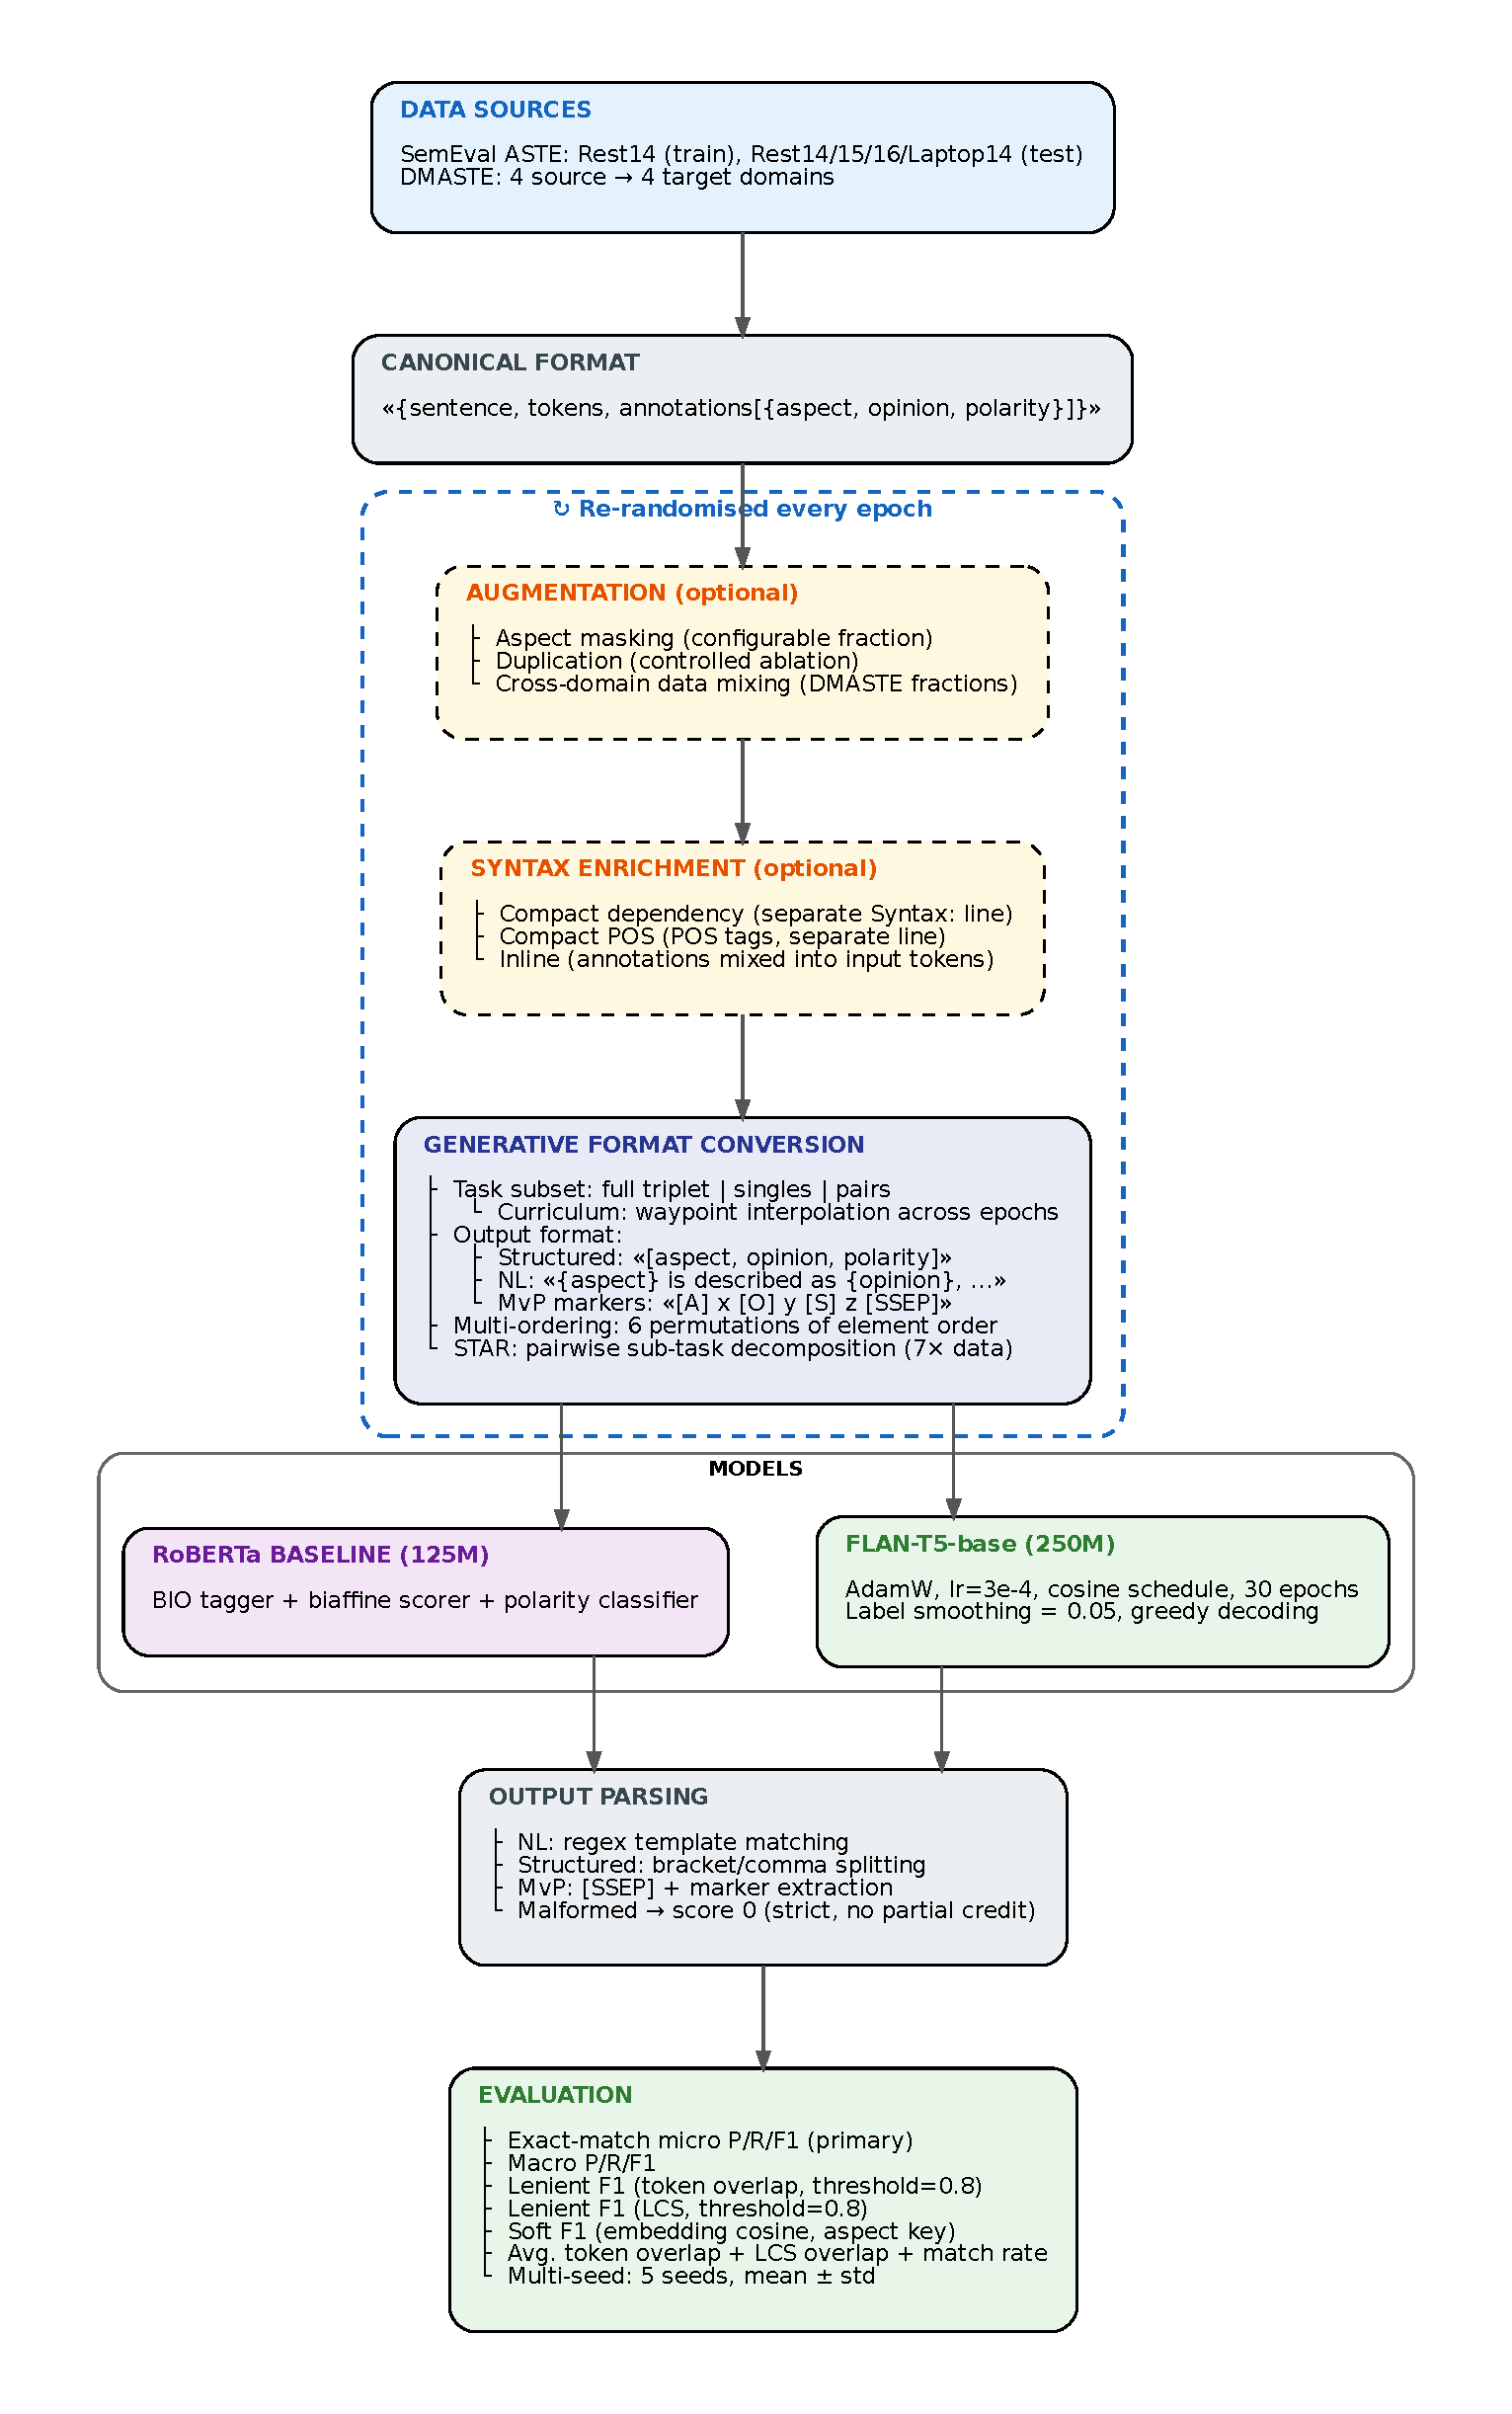
\includegraphics[width=\textwidth, height=0.88\textheight, keepaspectratio]{figures/pipeline_report3.pdf}
\caption{Training and evaluation pipeline. The dashed cluster indicates steps that are re-randomised every epoch.}
\label{fig:pipeline}
\end{figure}



\chapter{Experimental Results}\label{ch:results}

\section{Data Analysis}\label{sec:data-analysis}

Before presenting experimental results, we analyse the characteristics of the datasets to understand what makes cross-domain transfer difficult. Figure~\ref{fig:r3-polarity} shows the polarity distribution across datasets, and Figure~\ref{fig:r3-sentlen} compares sentence length distributions between the training domain (Rest14) and the OOD target (Laptop14).

The Rest14 training set contains 1266 sentences with 2338 annotations (1.85 annotations per sentence on average). Sentences are relatively short: mean 17.3 words, median 16, with 95\% of sentences under 34 words. The vocabulary is small (2916 unique words). Aspect spans are overwhelmingly single-word (mean 1.38 words) and opinion spans even shorter (mean 1.17 words). The polarity distribution is skewed toward positive (72.4\%), with negative at 20.5\% and neutral at 7.1\%.

\begin{figure}[H]
\centering
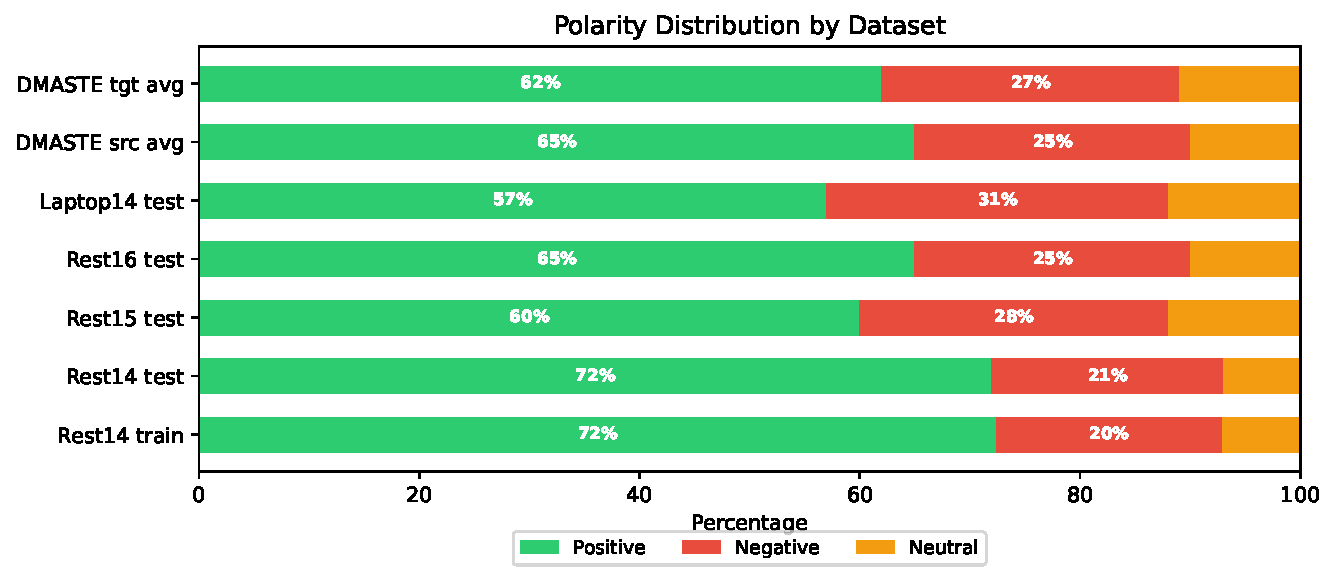
\includegraphics[width=0.95\textwidth]{figures/r3_polarity_distribution.pdf}
\caption{Polarity distribution across all datasets used in this report.}
\label{fig:r3-polarity}
\end{figure}

\begin{figure}[H]
\centering
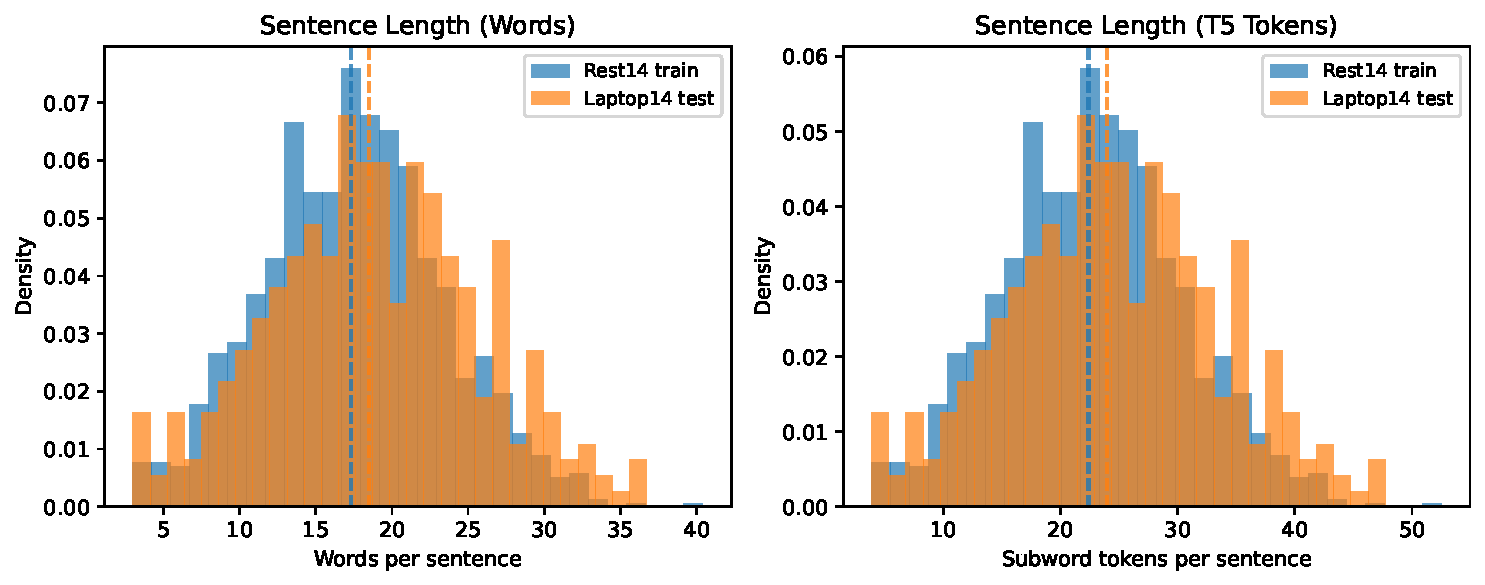
\includegraphics[width=0.95\textwidth]{figures/r3_sentence_length_histogram.pdf}
\caption{Sentence length distributions for Rest14 (training) and Laptop14 (OOD test) at word and subword token level.}
\label{fig:r3-sentlen}
\end{figure}

\subsection{Vocabulary Overlap}

Table~\ref{tab:vocab-overlap} shows token-level vocabulary overlap between training and test domains, measured separately for aspect and opinion terms. For SemEval, only 8.7\% of Laptop14 aspect tokens appear in the Rest14 training vocabulary, while the Rest14 test set shares 31\%. Opinion overlap is higher across the board: Laptop14 shares 47.3\% of opinion tokens with the training set, because words like ``good'', ``terrible'', ``excellent'' appear across domains while ``pizza'' and ``keyboard'' do not.

DMASTE target domains show higher overlap overall (24--55\% aspect, 60--76\% opinion) since they share the Amazon review style with the source domains. The Pet domain is an interesting case: it has the highest aspect overlap of any target (54.5\%) but second-worst F1, which points to vocabulary overlap being necessary but not sufficient for good cross-domain performance. We return to this in the structural characteristics section below.

\begin{table}[H]
\centering
\caption{Token-level vocabulary overlap (\%) between training and test domains. Aspect and opinion tokens measured separately.}
\label{tab:vocab-overlap}
\small
\begin{tabular}{@{}llcc@{}}
\toprule
\textbf{Train} & \textbf{Test} & \textbf{Aspect overlap} & \textbf{Opinion overlap} \\
\midrule
\multicolumn{4}{l}{\textit{SemEval (Rest14 train $\rightarrow$ test sets)}} \\
\midrule
Rest14 & Rest14 (ID) & 31.0 & 33.1 \\
Rest14 & Rest15 & 20.3 & 21.7 \\
Rest14 & Rest16 & 19.6 & 24.1 \\
Rest14 & Laptop14 (OOD) & 3.7 & 19.7 \\
\midrule
\multicolumn{4}{l}{\textit{DMASTE (source domains $\rightarrow$ target domains)}} \\
\midrule
Sources & Book & 24.4 & 60.2 \\
Sources & Grocery & 38.4 & 65.3 \\
Sources & Pet & 54.5 & 75.5 \\
Sources & Toy & 41.2 & 66.8 \\
\bottomrule
\end{tabular}
\end{table}

\subsection{Linguistic Differences}

The datasets differ in their annotation styles in ways that go beyond vocabulary. Figure~\ref{fig:pos-comparison} compares the POS tag distribution for opinion spans across all datasets. The most striking difference is in opinion annotations: SemEval opinions are adjective-dominant (37--46\% of opinion head POS tags are adjectives: ``delicious'', ``horrible''), while DMASTE opinions are verb-dominant (21--24\% verbs: ``works'', ``love'', ``recommend''). This reflects different annotation conventions rather than just different vocabulary. A model trained on adjective-heavy SemEval opinions may underperform on verb-heavy DMASTE opinions regardless of vocabulary overlap.

\begin{figure}[H]
\centering
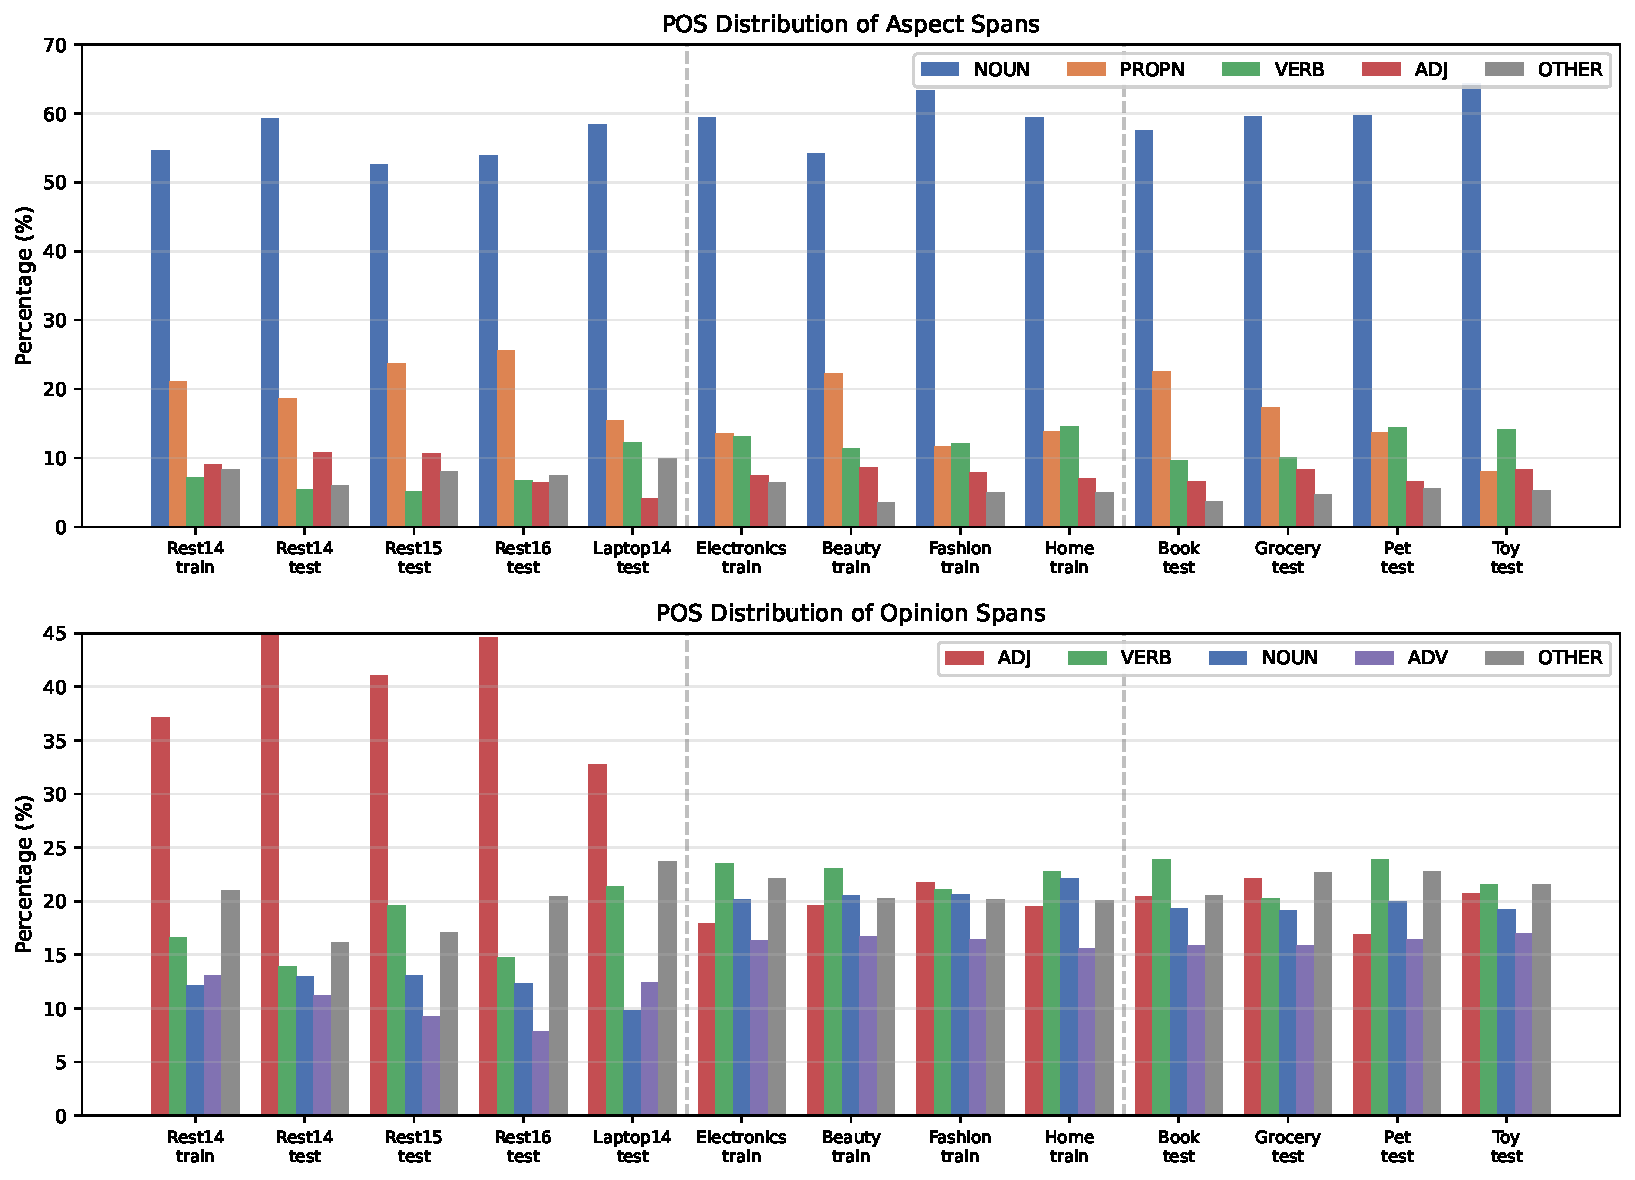
\includegraphics[width=0.95\textwidth]{figures/pos_comparison.pdf}
\caption{POS tag distribution for aspect terms (top) and opinion terms (bottom) across SemEval and DMASTE datasets. SemEval opinions are adjective-dominant while DMASTE opinions are verb-dominant.}
\label{fig:pos-comparison}
\end{figure}

\subsection{Structural Characteristics}

Table~\ref{tab:dataset-structure} summarises the structural differences between SemEval and DMASTE datasets. DMASTE sentences are 3--4$\times$ longer than SemEval (55--64 tokens vs 15--17), contain 2$\times$ more triplets per sentence (3.3--4.0 vs 1.5--2.0), and have much higher implicit aspect rates (38--47\% vs 0\% in SemEval). These compounding differences make DMASTE a substantially harder cross-domain target.

\begin{table}[H]
\centering
\caption{Structural characteristics of SemEval and DMASTE datasets.}
\label{tab:dataset-structure}
\small
\begin{tabular}{@{}lccccc@{}}
\toprule
\textbf{Dataset} & \textbf{Sentences} & \textbf{Mean length} & \textbf{Ann./sent.} & \textbf{Implicit \%} \\
\midrule
\multicolumn{5}{l}{\textit{SemEval}} \\
\midrule
Rest14 train & 1266 & 17.3 & 1.85 & 0\% \\
Rest14 test & 492 & 16.3 & 2.02 & 0\% \\
Rest15 test & 322 & 15.6 & 1.51 & 0\% \\
Rest16 test & 326 & 14.7 & 1.58 & 0\% \\
Laptop14 test & 328 & 15.8 & 1.66 & 0\% \\
\midrule
\multicolumn{5}{l}{\textit{DMASTE}} \\
\midrule
Electronics (source) & 1395 & 61.2 & 3.79 & 40.5\% \\
Beauty (source) & 535 & 58.8 & 4.15 & 43.6\% \\
Fashion (source) & 851 & 53.8 & 3.81 & 43.9\% \\
Home (source) & 1050 & 62.2 & 3.67 & 42.8\% \\
Book (target) & 325 & 55.4 & 3.29 & 37.8\% \\
Grocery (target) & 353 & 55.6 & 3.63 & 40.1\% \\
Pet (target) & 340 & 64.3 & 3.25 & 47.4\% \\
Toy (target) & 354 & 63.1 & 4.04 & 42.7\% \\
\bottomrule
\end{tabular}
\end{table}

The relationship between vocabulary overlap and performance is not straightforward. While overlap is necessary for good cross-domain F1, it is not sufficient: the Pet domain has the highest overlap with training sources but its 47.4\% implicit aspect rate (the highest of any domain) drags performance down regardless.


\section{Output Format Comparison}\label{sec:format-results}

Table~\ref{tab:format-5seed} presents the main result of this report: the comparison between structured and natural-language output format across 5 random seeds.

\begin{table}[H]
\centering
\caption{Output format comparison (5-seed mean$\pm$std, triplet micro-F1, Rest14-only training).}
\label{tab:format-5seed}
\small
\begin{tabular}{@{}lcccc@{}}
\toprule
\textbf{Configuration} & \textbf{Rest14 (ID)} & \textbf{Rest15} & \textbf{Rest16} & \textbf{Laptop14 (OOD)} \\
\midrule
Structured baseline & 0.693$\pm$0.008 & 0.575$\pm$0.009 & 0.640$\pm$0.009 & 0.439$\pm$0.012 \\
Structured + compact dep. & 0.699$\pm$0.004 & 0.578$\pm$0.012 & 0.655$\pm$0.008 & 0.447$\pm$0.012 \\
\midrule
NL baseline & 0.722$\pm$0.005 & \textbf{0.602$\pm$0.004} & 0.680$\pm$0.010 & \textbf{0.525$\pm$0.012} \\
NL + compact dep. & 0.708$\pm$0.006 & 0.596$\pm$0.006 & 0.669$\pm$0.004 & 0.509$\pm$0.005 \\
NL + compact POS & 0.699$\pm$0.003 & 0.601$\pm$0.010 & 0.672$\pm$0.007 & 0.506$\pm$0.012 \\
NL + mixed-objective & \textbf{0.730$\pm$0.005} & 0.593$\pm$0.010 & \textbf{0.686$\pm$0.009} & 0.524$\pm$0.011 \\
\bottomrule
\end{tabular}
\end{table}

The NL format provides +8.6 F1 points on OOD data over structured output (0.525 vs 0.439), with non-overlapping confidence intervals. The improvement comes entirely from the format switch: +2.9 F1 on Rest14, +2.7 on Rest15, +4.0 on Rest16, and +8.6 on Laptop14, with the gap widening as domain distance increases. Once the model uses NL output, adding syntax enrichment or mixed-objective training on top does not produce further gains: all NL variants land between 0.506 and 0.525 on Laptop14, within overlapping confidence intervals of each other. We believe the format advantage comes from alignment with FLAN-T5's pre-training distribution: on OOD data where the model has less task-specific confidence, generating fluent template sentences is something it can still fall back on, while producing correctly-structured bracket sequences requires a precision that degrades with domain shift.

\begin{figure}[H]
\centering
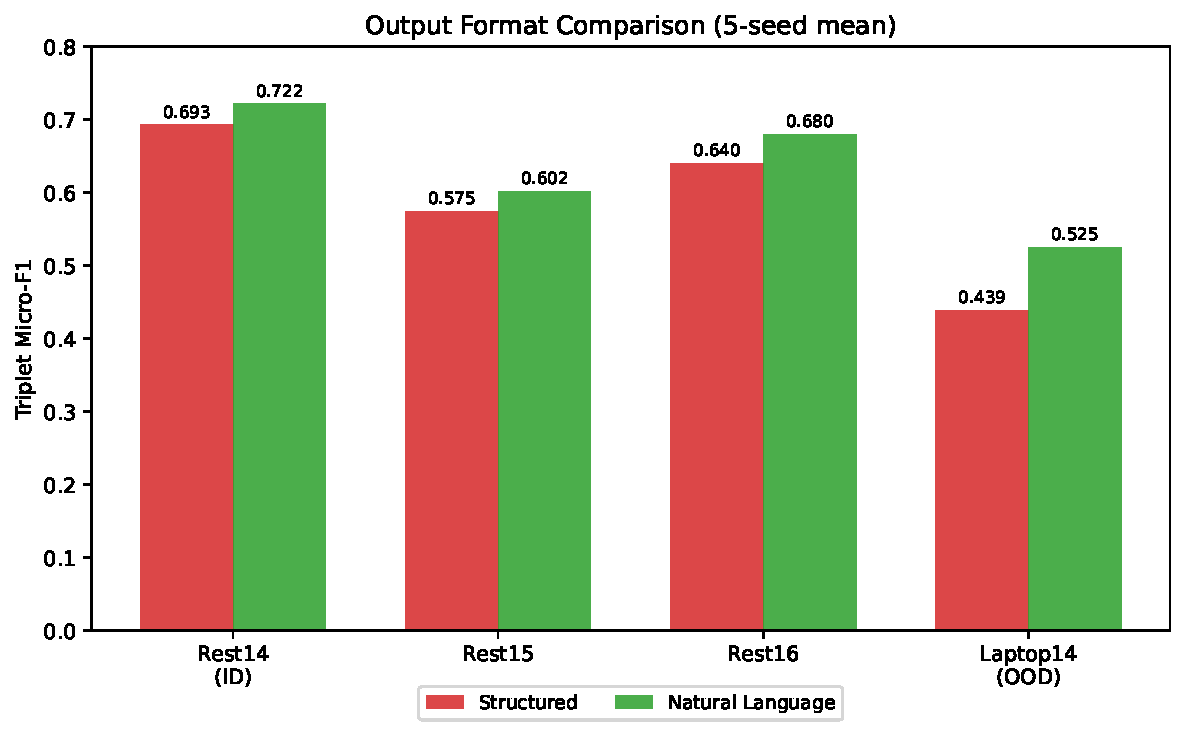
\includegraphics[width=0.85\textwidth]{figures/r3_output_format_comparison.pdf}
\caption{Output format comparison: structured vs natural-language F1 across all test sets (5-seed mean).}
\label{fig:r3-format}
\end{figure}


\section{Syntax Enrichment}\label{sec:syntax-results}

% Table~\ref{tab:format-5seed} already shows that compact dependency and compact POS annotations do not 
% significantly help OOD when combined with NL format. Table~\ref{tab:syntax-inline} shows additional 
% results for inline annotation modes.

Here we present the complete results for all syntactic enrichment approaches. 

\begin{table}[H]
\centering
\caption{Syntax modes comparison (triplet micro-F1, 20 epochs, structured format, Rest14-only training, seed 42).}
\label{tab:syntax-inline}
\small
\begin{tabular}{@{}lcc@{}}
\toprule
\textbf{Configuration} & \textbf{Rest14 (ID)} & \textbf{Laptop14 (OOD)} \\
\midrule
Baseline (no syntax) & 0.705 & 0.424 \\
+ inline dep. & 0.656 & 0.412 \\
+ inline POS & 0.660 & 0.382 \\
+ compact dep. & 0.708 & 0.481 \\
+ compact POS & 0.713 & 0.494 \\
\bottomrule
\end{tabular}
\end{table}

Table~\ref{tab:syntax-inline} reports triplet micro-F1 for all syntax annotation modes in the structured output format. Both inline modes hurt performance: inline dep drops OOD by 1.2 points and inline POS by 4.2 points relative to the baseline. When annotations are spliced directly into the input sequence, the model cannot easily distinguish annotation tokens from actual sentence content, and the effective input becomes noisier. The compact modes, which add syntax as a separate line after the sentence, avoid this interference and show modest OOD gains: +5.7 for compact dep and +7.0 for compact POS. However, as shown in the multi-seed evaluation with NL format in Table~\ref{tab:format-5seed}, these gains do not hold up to statistical testing once the NL format is applied.


\section{MvP and STAR Replications}\label{sec:mvp-star}

The following replications use seed 42. Results are compared against the 5-seed NL baseline from Section~\ref{sec:format-results}.

\begin{table}[H]
\centering
\caption{MvP and STAR replication results (triplet micro-F1, seed 42, Rest14-only training).}
\label{tab:mvp-star}
\small
\begin{tabular}{@{}lcccc@{}}
\toprule
\textbf{Configuration} & \textbf{Rest14} & \textbf{Rest15} & \textbf{Rest16} & \textbf{Laptop14} \\
\midrule
NL baseline (5-seed avg) & 0.722 & 0.602 & 0.680 & 0.525 \\
\midrule
MvP proper (greedy) & 0.728 & \textbf{0.605} & 0.688 & 0.528 \\
MvP proper + voting (thresh=3) & \textbf{0.735} & 0.604 & 0.693 & \textbf{0.530} \\
STAR proper (greedy) & 0.718 & 0.592 & 0.692 & 0.487 \\
STAR proper + voting (thresh=3) & 0.723 & 0.598 & \textbf{0.714} & 0.500 \\
\midrule
NL + multi-ordering (5-seed) & 0.730 & 0.593 & 0.686 & 0.524 \\
\bottomrule
\end{tabular}
\end{table}

Table~\ref{tab:mvp-star} reports triplet micro-F1 for the MvP and STAR replications. MvP with majority voting achieves 0.530 on Laptop14, which is 0.5 points above the 5-seed NL baseline mean (0.525) but well within its confidence interval ($\pm$0.012). The voting mechanism provides a clearer benefit in-domain (+1.3 points on Rest14), where it helps resolve ambiguous element orderings. On OOD data, however, the errors come from vocabulary mismatch rather than compositional ambiguity, so voting over multiple orderings of the same incorrect prediction does not help.

STAR shows a different pattern: Laptop14 drops to 0.487 (greedy) and 0.500 (with voting), both below the baseline by 2.5--3.8 points. STAR's data multiplication generates additional training instances (pairwise relations like aspect+opinion, aspect+polarity) from the same restaurant-domain data. This increases the total training signal by roughly 7$\times$ but all of it is drawn from the same distribution. We believe the OOD degradation occurs because the model spends more capacity learning fine-grained pairwise patterns specific to restaurant vocabulary rather than building general representations that could transfer to laptop reviews.


\section{Negative Results}\label{sec:negative}

The ablation studies in Sections~\ref{sec:curriculum}--\ref{sec:decoding} use a single random seed (42) to reduce computational cost. The NL baseline for seed 42 alone is Rest14 = 0.727, Laptop14 = 0.543, which falls within the 5-seed distribution reported in Section~\ref{sec:format-results} (0.722$\pm$0.005 and 0.525$\pm$0.012 respectively). Results are compared against the 5-seed mean to provide context, but the single-seed ablations should be interpreted as directional evidence rather than statistically validated findings.

\subsection{Curriculum Learning}\label{sec:curriculum}

\begin{table}[H]
\centering
\caption{Curriculum learning results (triplet micro-F1, 28 epochs, NL format, Rest14 training, seed 42).}
\label{tab:curriculum}
\small
\begin{tabular}{@{}lcccc@{}}
\toprule
\textbf{Schedule} & \textbf{Rest14 (ID)} & \textbf{Rest15} & \textbf{Rest16} & \textbf{Laptop14 (OOD)} \\
\midrule
NL baseline (5-seed avg) & 0.722 & 0.602 & 0.680 & 0.525 \\
\midrule
Overlap-first & 0.716 & 0.577 & 0.670 & 0.502 \\
Fast ramp & 0.722 & 0.593 & 0.673 & 0.509 \\
Sandwich & 0.713 & 0.612 & 0.680 & 0.507 \\
\bottomrule
\end{tabular}
\end{table}

Table~\ref{tab:curriculum} reports triplet micro-F1 for three curriculum schedules. All three drop Laptop14 performance by 1.6--2.3 points relative to the 5-seed baseline (0.525): overlap-first reaches 0.502, fast ramp 0.509, and sandwich 0.507. On in-domain data the differences are small, and the sandwich schedule actually achieves the best Rest15 result (0.612 vs baseline 0.602), suggesting some regularisation benefit for near-OOD transfer within the restaurant domain family.

The common pattern is that curriculum schedules control the order in which the model transitions from simpler objectives to full triplet prediction, but all training data still comes from the restaurant domain. The schedules affect how quickly the model converges on in-domain patterns, not what features it learns. Since OOD performance depends on learning domain-general representations (vocabulary-independent syntactic patterns, polarity cues) rather than on the training trajectory, rearranging when the model sees what type of training signal does not address the core challenge.

\subsection{Aspect Masking}\label{sec:masking}

\begin{table}[H]
\centering
\caption{Aspect masking results (triplet micro-F1, NL format, 28 epochs, Rest14 training, seed 42). Mask fraction = 20\%.}
\label{tab:masking}
\small
\begin{tabular}{@{}lcccc@{}}
\toprule
\textbf{Configuration} & \textbf{Rest14 (ID)} & \textbf{Rest15} & \textbf{Rest16} & \textbf{Laptop14 (OOD)} \\
\midrule
NL baseline (5-seed avg) & 0.722 & 0.602 & 0.680 & 0.525 \\
\midrule
Mask 20\% & 0.710 & 0.598 & 0.671 & 0.518 \\
Mask 20\% + dep. & 0.705 & 0.598 & 0.675 & 0.511 \\
\bottomrule
\end{tabular}
\end{table}

Table~\ref{tab:masking} shows that masking hurts triplet micro-F1 across all test sets. At 20\% mask fraction, Laptop14 drops from 0.525 to 0.518, and adding dependency annotations on top brings it further down to 0.511. Rest15 and Rest16 show similar, smaller degradation (0.598 and 0.671/0.675 vs baseline 0.602 and 0.680). The original premise was that replacing aspect spans with sentinel tokens would force the model to rely on contextual cues rather than copying, which should help when test-time aspects are novel. In practice, we suspect the opposite happens: during training on restaurant data, the model learns to infer masked aspects from surrounding restaurant vocabulary (e.g. predicting ``food'' or ``service'' when context mentions taste or waiting), which reinforces domain-specific priors rather than building domain-general representations. At test time in the laptop domain, those same priors produce incorrect predictions because the contextual cues are different.

\subsection{Cross-Domain Data Mixing}\label{sec:domainmix}

\begin{table}[H]
\centering
\caption{Domain mixing results (triplet micro-F1, Rest14 + DMASTE domain fraction, seed 42). The NL baseline's 5-seed confidence interval for Laptop14 is 0.525$\pm$0.012.}
\label{tab:domainmix}
\small
\begin{tabular}{@{}lcccc@{}}
\toprule
\textbf{Mixed domain} & \textbf{Rest14} & \textbf{Rest15} & \textbf{Rest16} & \textbf{Laptop14} \\
\midrule
None (baseline) & 0.727 & 0.607 & 0.672 & 0.543 \\
\midrule
+ Beauty & 0.707 & 0.610 & 0.699 & 0.523 \\
+ Electronics & 0.720 & 0.605 & 0.685 & 0.526 \\
+ Fashion & 0.709 & 0.589 & 0.689 & 0.502 \\
+ Home & 0.736 & 0.596 & 0.689 & 0.525 \\
+ All four & 0.719 & 0.615 & 0.668 & 0.522 \\
\bottomrule
\end{tabular}
\end{table}

Table~\ref{tab:domainmix} reports triplet micro-F1 for each domain mixing configuration. All Laptop14 results (0.502--0.526) fall within the 5-seed baseline confidence interval (0.525$\pm$0.012), meaning no variant is distinguishable from training on Rest14 alone. The ``+All four'' configuration does improve Rest15 (0.615 vs 0.607 baseline), suggesting that adding diverse product-review data helps transfer within the same review-style family (Amazon-like sentences).

The lack of far-OOD improvement is likely explained by what the mixed data actually provides. DMASTE domains share annotation conventions, sentence structure, and review style with each other (long multi-aspect Amazon reviews) but differ substantially from SemEval (short single-topic Yelp sentences). Adding more Amazon-style data from beauty, electronics, fashion, or home categories diversifies the product vocabulary but does not bridge the structural and stylistic gap between Amazon reviews and SemEval laptop reviews. For domain mixing to help far-OOD, the added data would need to resemble the target domain in structure, not just provide more diverse aspect terms.

\subsection{Decoding Strategies}\label{sec:decoding}

\begin{table}[H]
\centering
\caption{Decoding strategies (triplet micro-F1, NL format with compact dependency annotations, seed 42).}
\label{tab:decoding}
\small
\begin{tabular}{@{}lcc@{}}
\toprule
\textbf{Strategy} & \textbf{Rest14 (ID)} & \textbf{Laptop14 (OOD)} \\
\midrule
Greedy (default) & 0.708 & 0.541 \\
Beam search (k=4) & 0.713 & 0.530 \\
Sampling (t=0.7) & 0.699 & 0.477 \\
Sampling (t=0.9) & 0.672 & 0.446 \\
Voting (5$\times$, t=0.8) & 0.710 & 0.520 \\
Constrained decoding & 0.699 & 0.483 \\
\bottomrule
\end{tabular}
\end{table}

Table~\ref{tab:decoding} reports triplet micro-F1 for several decoding strategies, all applied at 
test time to the same trained checkpoint (NL + compact dep., seed 42). Out of all decoding strategies tested, greedy decoding achieves 
the best OOD result of 0.541. Beam search (k=4) also provides a small ID gain of 0.5, however it drops 
OOD F1 by 1.1 points. 
Temperature sampling is shown to degrade performance substantially. A temperature of 0.7 loses 6.4 points OOD 
and a temperature of 0.9 loses 9.5 points. Voting over 5 samples recovers partially, achieving 0.71 ID and 0.52 OOD
but is still significantly behind greedy decoding in both ID and OOD setting.

\begin{figure}[H]
\centering
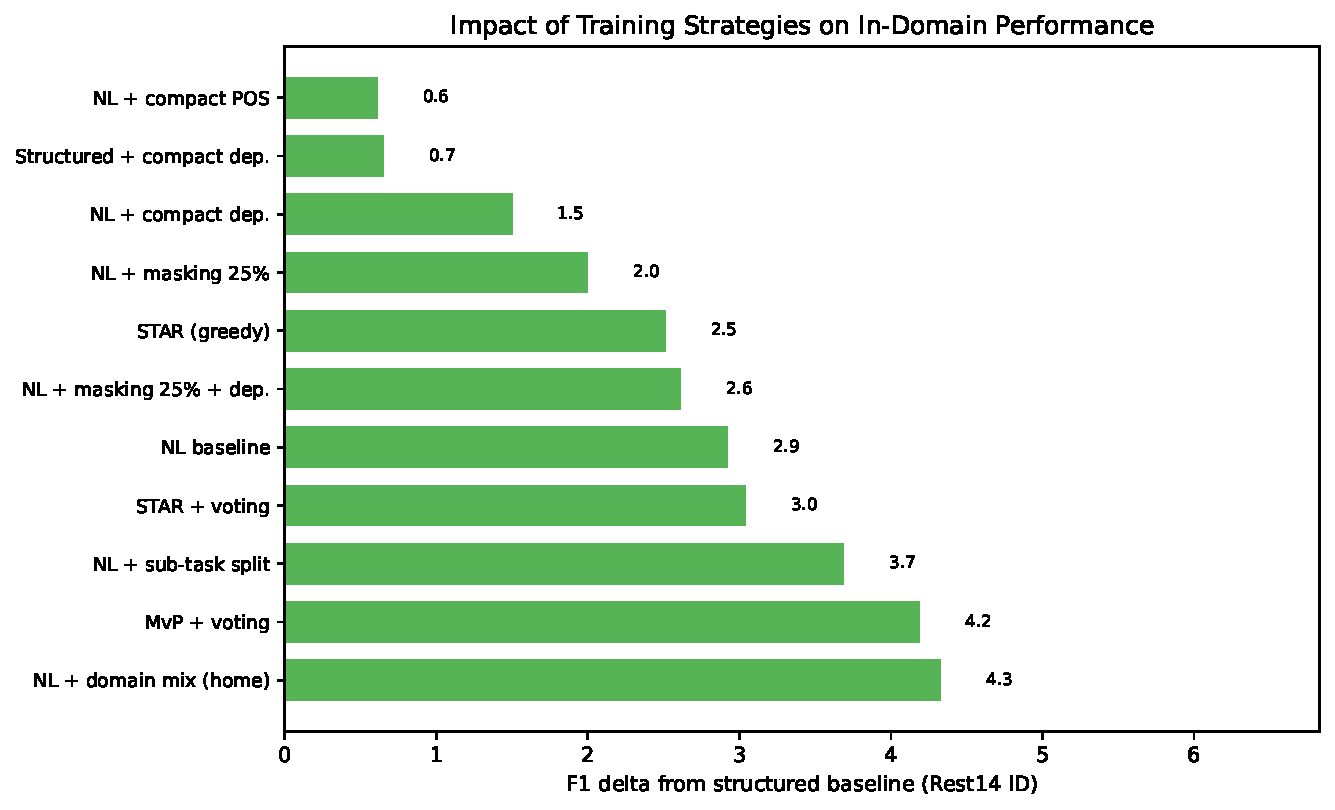
\includegraphics[width=0.95\textwidth]{figures/r3_id_results_tornado.pdf}
\caption{F1 improvement over the structured baseline for each training strategy on Rest14 (ID).}
\label{fig:r3-id-tornado}
\end{figure}

\begin{figure}[H]
\centering
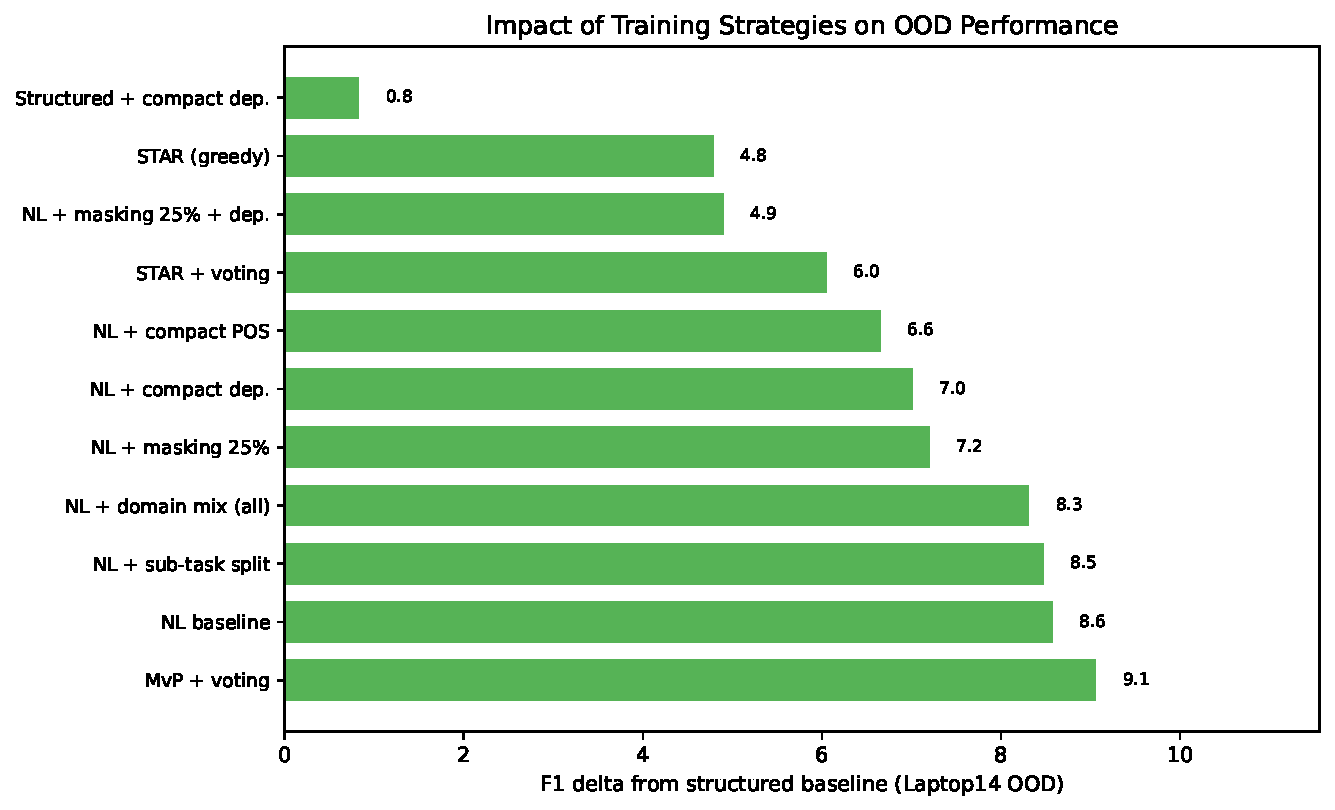
\includegraphics[width=0.95\textwidth]{figures/r3_negative_results_tornado.pdf}
\caption{F1 improvement over the structured baseline for each training strategy on Laptop14 (OOD).}
\label{fig:r3-ood-tornado}
\end{figure}

Figures~\ref{fig:r3-id-tornado} and~\ref{fig:r3-ood-tornado} summarise the impact of all tested strategies relative to the structured baseline. On ID data, most NL-based strategies provide 2--4 F1 points of improvement. On OOD data, the NL baseline provides the largest gain (+8.6), while strategies like STAR and masking provide smaller improvements over structured but do not add value beyond the NL format itself.


\section{DMASTE Cross-Domain Benchmark}\label{sec:dmaste}

\begin{table}[H]
\centering
\caption{DMASTE cross-domain results (triplet micro-F1, single seed).}
\label{tab:dmaste}
\small
\begin{tabular}{@{}lccccc@{}}
\toprule
\textbf{Method} & \textbf{Book} & \textbf{Grocery} & \textbf{Pet} & \textbf{Toy} & \textbf{Avg} \\
\midrule
\multicolumn{6}{l}{\textit{Single-source (Electronics $\rightarrow$ target)}} \\
\midrule
Structured & 34.49 & 38.88 & 37.62 & 44.67 & 38.92 \\
NL baseline & 36.05 & 43.65 & 38.93 & 46.74 & 41.34 \\
NL + multi-ordering & 37.28 & 43.78 & 40.33 & 46.72 & 42.03 \\
NL + compact dep. & 34.74 & 42.45 & 38.47 & 44.77 & 40.11 \\
RoBERTa (span) & 10.59 & 16.08 & 15.35 & 13.95 & 13.99 \\
\midrule
GAS$^\dagger$~\cite{zhang2021towards} & 35.57 & 39.16 & 38.17 & 43.55 & 39.11 \\
Span-ASTE$^\dagger$~\cite{xu2021learning} & \textbf{40.36} & \textbf{45.36} & \textbf{41.04} & \textbf{47.23} & \textbf{43.50} \\
\midrule
\multicolumn{6}{l}{\textit{Multi-source (All 4 sources $\rightarrow$ target)}} \\
\midrule
Structured & 37.50 & 44.96 & 42.47 & 47.33 & 43.07 \\
NL baseline & 41.27 & 46.62 & 43.22 & 50.16 & 45.32 \\
NL + multi-ordering & \textbf{41.83} & \textbf{46.90} & 43.06 & 50.02 & \textbf{45.45} \\
NL + compact dep. & 40.45 & 46.47 & \textbf{43.77} & 48.56 & 44.81 \\
RoBERTa (span) & 20.39 & 23.16 & 22.37 & 22.15 & 22.02 \\
\midrule
Span-ASTE$^\dagger$~\cite{xu2021learning} & \textbf{41.83} & 46.07 & 43.62 & \textbf{50.16} & 45.42 \\
\bottomrule
\multicolumn{6}{l}{\small $^\dagger$ Results as reported by Xu et al.~\cite{xu2023dmaste}.}
\end{tabular}
\end{table}

In the multi-source setting, our NL models (45.32--45.45 avg) match Span-ASTE (45.42), the best result reported in the DMASTE paper~\cite{xu2023dmaste}. This is achieved without any domain adaptation, using a simple FLAN-T5-base model with NL output. In single-source, we outperform GAS (+3 avg F1) and approach Span-ASTE ($-$1.5 avg).

The NL format advantage over structured output (+2.3 avg in multi-source) is smaller than on SemEval (+8.6) but consistent. Syntax enrichment does not help on DMASTE (slightly negative), consistent with SemEval findings.

The RoBERTa span baseline generalises very poorly to DMASTE (14--22 avg), confirming that our naive discriminative implementation lacks cross-domain transfer capability. Published discriminative methods like Span-ASTE, which use specialised architectures, perform considerably better (43.50--45.42 avg).

\begin{figure}[H]
\centering
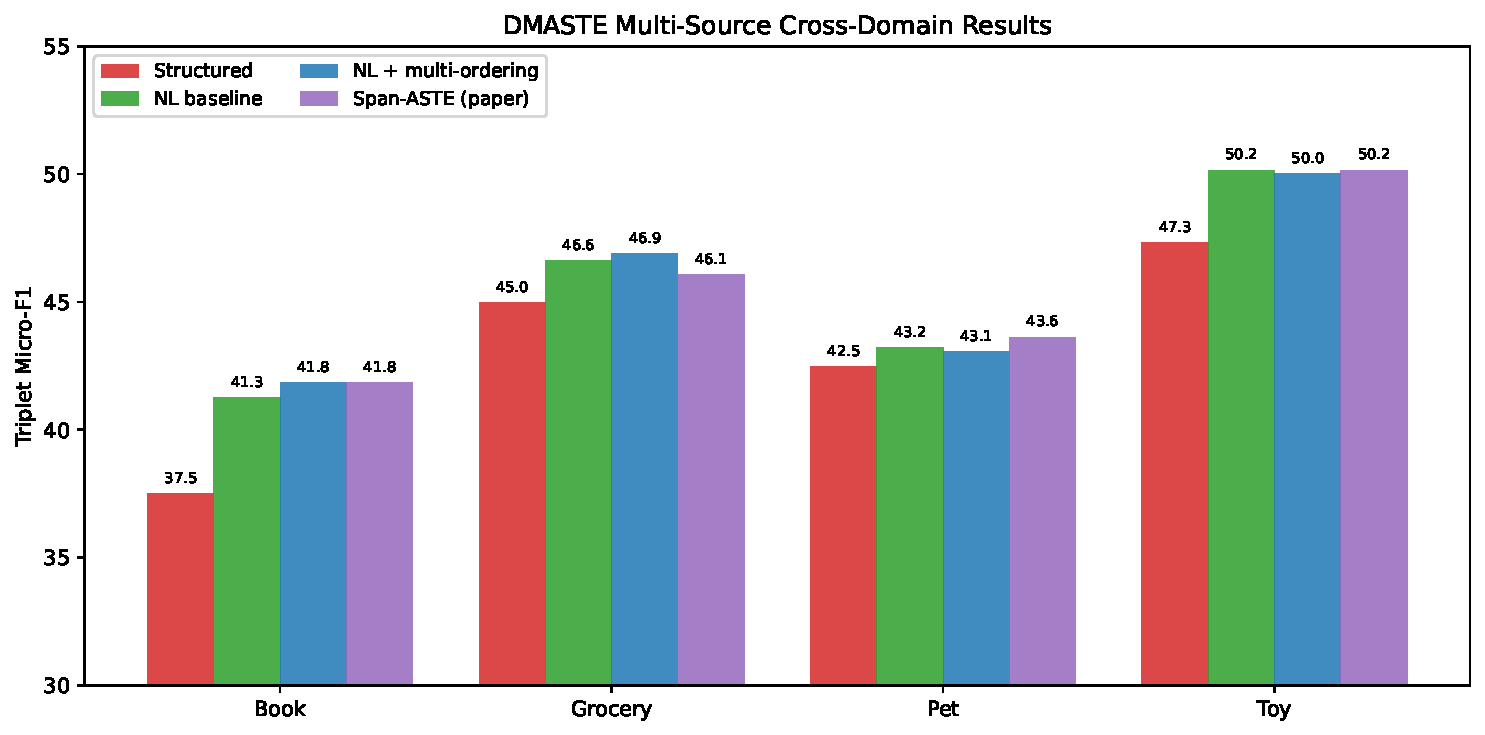
\includegraphics[width=0.95\textwidth]{figures/r3_dmaste_comparison.pdf}
\caption{DMASTE multi-source cross-domain results by method and target domain.}
\label{fig:r3-dmaste}
\end{figure}


\section{Error Analysis}\label{sec:errors}

To understand where the model fails on out-of-domain data and how those failures compare to in-domain performance, we ran a detailed error classification on the NL baseline (seed 42) for both Rest14 (ID, F1 = 0.725) and Laptop14 (OOD, F1 = 0.542). For each unmatched prediction, we classified errors at the element level (aspect, opinion, and polarity independently) and at the triplet level (which combination of elements is wrong). For each missed gold, we checked whether the aspect and opinion terms had been seen during training.

\subsection{Element-Level Errors}

\begin{table}[H]
\centering
\caption{Element-level error classification for unmatched predictions on Rest14 (ID) and Laptop14 (OOD). Percentages are relative to the total number of errors in each category.}
\label{tab:errors-element}
\small
\begin{tabular}{@{}lrrrr@{}}
\toprule
& \multicolumn{2}{c}{\textbf{Rest14 (ID)}} & \multicolumn{2}{c}{\textbf{Laptop14 (OOD)}} \\
\textbf{Error type} & \textbf{Count} & \textbf{\%} & \textbf{Count} & \textbf{\%} \\
\midrule
\multicolumn{5}{l}{\textit{Aspect errors}} \\
\midrule
Spurious & 81 & 57.4 & 115 & 81.6 \\
Boundary & 55 & 39.0 & 20 & 14.2 \\
Paraphrase & 4 & 2.8 & 1 & 0.7 \\
Hallucination & 1 & 0.7 & 5 & 3.5 \\
\midrule
\multicolumn{5}{l}{\textit{Opinion errors}} \\
\midrule
Spurious & 100 & 70.4 & 73 & 68.2 \\
Boundary & 42 & 29.6 & 33 & 30.8 \\
Hallucination & 0 & 0.0 & 1 & 0.9 \\
\midrule
\multicolumn{5}{l}{\textit{Polarity errors}} \\
\midrule
Wrong polarity & 130 & --- & 126 & --- \\
\bottomrule
\end{tabular}
\end{table}

Table~\ref{tab:errors-element} shows a notable shift in error composition between in-domain and out-of-domain evaluation. On Rest14, aspect boundary errors account for 39\% of aspect mistakes, which suggests that when the model operates within a familiar domain it tends to identify the correct region of the sentence but disagrees on which words exactly constitute the span (for instance predicting ``grilled chicken'' where the gold is just ``chicken''). On Laptop14, boundary errors drop to 14.2\% while spurious errors rise from 57.4\% to 81.6\%, which we interpret as the model extracting real text from the sentence that happens not to correspond to any annotated aspect. Many of these spurious extractions appear to involve adjectives or verbs in aspect-like syntactic positions that would not be annotated as aspects under the SemEval guidelines (examples in the data include ``fast'', ``light'', ``compatible'').

Opinion errors appear to be more stable across domains, with spurious extractions at 70.4\% in-domain and 68.2\% OOD, and boundary errors at roughly 30\% in both cases. This relative stability is consistent with the vocabulary overlap numbers in Table~\ref{tab:vocab-overlap}, where opinion token overlap between Rest14 and Laptop14 is considerably higher than aspect overlap.

\subsection{Triplet-Level Error Patterns}

\begin{table}[H]
\centering
\caption{Triplet-level error patterns: which element combinations are wrong in unmatched predictions.}
\label{tab:errors-triplet}
\small
\begin{tabular}{@{}lrrrr@{}}
\toprule
& \multicolumn{2}{c}{\textbf{Rest14 (ID)}} & \multicolumn{2}{c}{\textbf{Laptop14 (OOD)}} \\
\textbf{Pattern} & \textbf{Count} & \textbf{\%} & \textbf{Count} & \textbf{\%} \\
\midrule
aspect+opinion+polarity & 70 & 25.9 & 71 & 33.0 \\
aspect only & 63 & 23.3 & 58 & 27.0 \\
opinion only & 63 & 23.3 & 26 & 12.1 \\
polarity only & 43 & 15.9 & 33 & 15.3 \\
aspect+polarity & 8 & 3.0 & 12 & 5.6 \\
opinion+polarity & 9 & 3.3 & 10 & 4.7 \\
duplicate & 14 & 5.2 & 5 & 2.3 \\
\bottomrule
\end{tabular}
\end{table}

Table~\ref{tab:errors-triplet} breaks down the same errors by which combination of elements is wrong in each unmatched prediction. On in-domain data, the distribution is relatively even between aspect-only (23.3\%), opinion-only (23.3\%), and all-three-wrong (25.9\%), with no single element appearing to be the dominant bottleneck. On OOD data the balance shifts: opinion-only errors drop from 23.3\% to 12.1\%, which is consistent with opinion vocabulary being more transferable, while aspect-only errors grow slightly to 27\% and the all-three-wrong pattern rises to 33\%. We believe this last category largely represents cases where the model has pointed at an entirely unrelated part of the sentence, producing an aspect, opinion, and polarity that bear no relation to any gold triplet.

\subsection{Missed Extractions}

\begin{table}[H]
\centering
\caption{Classification of missed gold triplets by whether the aspect/opinion terms appeared in training.}
\label{tab:errors-missed}
\small
\begin{tabular}{@{}lrrrr@{}}
\toprule
& \multicolumn{2}{c}{\textbf{Rest14 (ID)}} & \multicolumn{2}{c}{\textbf{Laptop14 (OOD)}} \\
\textbf{Missed type} & \textbf{Count} & \textbf{\%} & \textbf{Count} & \textbf{\%} \\
\midrule
Aspect unseen in training & 147 & 53.5 & 254 & 97.3 \\
Aspect seen in training & 128 & 46.5 & 7 & 2.7 \\
\midrule
Opinion unseen in training & 95 & 34.5 & 131 & 50.2 \\
Opinion seen in training & 180 & 65.5 & 130 & 49.8 \\
\bottomrule
\end{tabular}
\end{table}

Table~\ref{tab:errors-missed} provides what we consider the clearest evidence for why OOD performance drops. On Laptop14, 97.3\% of missed gold aspects are terms that never appeared in the restaurant training data (words like ``OS'', ``trackpad'', ``portability'', ``setup''), which leaves the model with no learned association between these tokens and the concept of ``aspect.'' The 2.7\% of missed aspects that were seen in training tend to be domain-general terms like ``price'' or ``quality'' that the model occasionally fails to extract in the unfamiliar laptop context.

As far as opinion terms are concerned, on Laptop14, the split between unseen and seen is nearly even at 50.2\% vs 49.8\%, consistent with the higher opinion token overlap reported in Section~\ref{sec:data-analysis}. This suggests that when the model misses an opinion on OOD data, the issue is less about never having seen the word and more about failing to recognise it as an opinion, due to the different context.

\subsection{Annotation Quality}

A non-trivial fraction of what the evaluation counts as errors are debatable annotations rather than genuine model failures:

\begin{itemize}
    \item Hypotheticals labelled as opinions: ``a spice rub \textit{might have} overwhelmed'' is annotated as a negative opinion about spice rub, despite being a hypothetical dismissal where the reviewer is explaining why the chef avoided something.
    \item Neutral labels in clearly opinionated contexts: ``There is no HDMI receptacle, nor is there an SD card slot located anywhere on the device'' is annotated as neutral, while the model predicts negative, which seems natural for a review statement about a missing feature.
\end{itemize}

We estimate that 5--10\% of Laptop14 annotations involve genuinely ambiguous polarity where the model's prediction is at least as defensible as the gold label. This affects all methods equally and does not change relative comparisons between strategies.



\chapter{Conclusions}\label{ch:conclusions}

\section{Summary}

This report presented an empirical study of training strategies for OOD generalisation in generative ABSA. We evaluated output format, syntactic enrichment, multi-ordering training, mixed-objective training, curriculum learning, aspect masking, cross-domain data mixing, and decoding strategies, measuring their OOD impact with multi-seed statistical validation on two benchmarks.

The main finding is that natural-language output format provides the largest improvement for OOD generalisation: +8.6 F1 points over structured output with non-overlapping confidence intervals across 5 seeds. This is a design choice that requires no additional data or computation, yet delivers larger OOD gains than any other intervention we tested. On the DMASTE benchmark, our model with NL output matches the best previously reported cross-domain result (Span-ASTE) without any domain adaptation techniques.

The remaining strategies we tested did not improve OOD F1 beyond the NL baseline's confidence interval of 0.525$\pm$0.012 on Laptop14. Compact syntax enrichment scored 0.509, mixed-objective training 0.524, curriculum learning 0.502--0.509, aspect masking 0.511--0.518, and cross-domain data mixing 0.502--0.526. On DMASTE, syntax similarly provided no gain over the NL baseline. We interpret this as evidence that the OOD bottleneck for our setup is the domain gap itself, specifically the vocabulary and annotation-style differences documented in Section~\ref{sec:data-analysis}, rather than insufficient training signal from the source domain.

\section{Future Work}

For our next report, ee plan to compare our fine-tuned model against LLMs in both 0-shot and few-shot settings, 
to determine the extent of the small model fine-tuning advantage relative to large pretrained models.
 We also plan to evaluate whether the natural language format advantage carries over to Romanian, 
 using a dataset of eMAG phone reviews annotated for aspect polarity and category.

On the augmentation side, based on the error analysis we performed (Section~\ref{sec:errors}), where
97\% of missed aspects as well as 50\% of missed opinions in OOD evaluation were terms 
unseen during training, we plan to build an LLM paraphrasing pipeline, for aspect and opinion terms,
to increase diversity of vocabulary without the need for additional datasets.

\chapter{Annex}\label{ch:annex}

\section{Per-Seed Results}

\begin{table}[H]
\centering
\caption{NL baseline: per-seed triplet F1 on all test sets (Rest14-only training).}
\small
\begin{tabular}{@{}ccccc@{}}
\toprule
\textbf{Seed} & \textbf{Rest14} & \textbf{Rest15} & \textbf{Rest16} & \textbf{Laptop14} \\
\midrule
42 & 0.727 & 0.607 & 0.672 & 0.543 \\
123 & 0.718 & 0.598 & 0.688 & 0.517 \\
456 & 0.717 & 0.603 & 0.672 & 0.520 \\
789 & 0.727 & 0.600 & 0.690 & 0.532 \\
1337 & 0.720 & 0.603 & 0.677 & 0.512 \\
\midrule
Mean & 0.722 & 0.602 & 0.680 & 0.525 \\
Std & 0.005 & 0.004 & 0.010 & 0.012 \\
\bottomrule
\end{tabular}
\end{table}

\begin{table}[H]
\centering
\caption{Structured baseline: per-seed triplet F1 (Rest14-only training).}
\small
\begin{tabular}{@{}ccccc@{}}
\toprule
\textbf{Seed} & \textbf{Rest14} & \textbf{Rest15} & \textbf{Rest16} & \textbf{Laptop14} \\
\midrule
42 & 0.698 & 0.570 & 0.637 & 0.421 \\
123 & 0.684 & 0.580 & 0.640 & 0.441 \\
456 & 0.694 & 0.565 & 0.632 & 0.449 \\
789 & 0.701 & 0.582 & 0.651 & 0.441 \\
1337 & 0.686 & 0.577 & 0.640 & 0.444 \\
\midrule
Mean & 0.693 & 0.575 & 0.640 & 0.439 \\
Std & 0.008 & 0.009 & 0.009 & 0.012 \\
\bottomrule
\end{tabular}
\end{table}

\section{Example Model Outputs}

\textbf{Correct extraction (ID, Rest14):}
\begin{lstlisting}
Input: Great food but the service was dreadful !
Output: food is described as Great, expressing a positive sentiment ;
        service is described as dreadful, expressing a negative sentiment
\end{lstlisting}

\textbf{OOD error --- unseen aspect (Laptop14):}
\begin{lstlisting}
Input: This Macbook Pro is fast, powerful, and runs super quiet and cool.
Gold: runs -> quiet [positive] ; runs -> cool [positive]
Pred: Macbook Pro -> fast [positive] ; Macbook Pro -> powerful [positive] ;
      Macbook Pro -> quiet [positive] ; Macbook Pro -> cool [positive]
\end{lstlisting}
The model identifies the product name as the aspect rather than the verb ``runs''. This reflects different annotation conventions between restaurant and laptop domains.

\textbf{OOD error --- polarity confusion (Laptop14):}
\begin{lstlisting}
Input: I needed a laptop with big storage, a nice screen and fast ...
Gold: storage -> big [neutral] ; screen -> nice [neutral]
Pred: storage -> big [positive] ; screen -> nice [positive]
\end{lstlisting}
Desire/wish context should be neutral per annotation guidelines, but the model defaults to positive for positive-sounding adjectives.

\section{Input/Output Format Examples}

\textbf{Full prompt with compact dependency annotations:}
\begin{lstlisting}
Task: aspect-extraction, sentiment-extraction, polarity-inference
Input: The staff was so horrible to us .
Syntax: staff->was:nsubj horrible->was:acomp
Output: staff is described as horrible, expressing a negative sentiment
\end{lstlisting}

\textbf{Structured output for the same input:}
\begin{lstlisting}
Task: aspect-extraction, sentiment-extraction, polarity-inference
Input: The staff was so horrible to us .
Output: [staff, horrible, negative]
\end{lstlisting}


\section{Multi-Ordering Template Permutations}\label{sec:annex-templates}

The 6 natural-language templates used for multi-ordering training on the full ASTE triplet task. Each permutation of the task prefix produces a different template:

\begin{table}[H]
\centering
\caption{NL output templates for all 6 element orderings of the ASTE triplet.}
\small
\begin{tabular}{@{}lp{10.5cm}@{}}
\toprule
\textbf{Task prefix order} & \textbf{Template} \\
\midrule
aspect, sentiment, polarity & \texttt{\{aspect\} is described as \{sentiment\}, expressing a \{polarity\} sentiment} \\
aspect, polarity, sentiment & \texttt{\{aspect\} carries a \{polarity\} opinion, expressed as \{sentiment\}} \\
sentiment, aspect, polarity & \texttt{the opinion \{sentiment\} is expressed towards \{aspect\}, conveying a \{polarity\} sentiment} \\
sentiment, polarity, aspect & \texttt{\{sentiment\} conveys a \{polarity\} sentiment about \{aspect\}} \\
polarity, aspect, sentiment & \texttt{a \{polarity\} sentiment toward \{aspect\} is expressed as \{sentiment\}} \\
polarity, sentiment, aspect & \texttt{a \{polarity\} sentiment is expressed as \{sentiment\}, regarding \{aspect\}} \\
\bottomrule
\end{tabular}
\end{table}

For example, with the sentence ``But the staff was so horrible to us'', the ordering (sentiment, aspect, polarity) produces:

\begin{lstlisting}
Task: sentiment-extraction, aspect-extraction, polarity-inference
Input: But the staff was so horrible to us .
Output: the opinion horrible is expressed towards staff, conveying a negative sentiment
\end{lstlisting}


\clearpage
\addcontentsline{toc}{chapter}{Bibliography}
\bibliographystyle{ieeetr}
\bibliography{bibliography3}

\end{document}
